%!TEX root = ../thesis.tex
%*******************************************************************************
%****************************** Second Chapter *********************************
%*******************************************************************************

\chapter{Results of Physical Properties Modification in Novel 2D materials \label{chap:5}}

\ifpdf
    \graphicspath{{Chapter5/Figs/Raster/}{Chapter5/Figs/PDF/}{Chapter5/Figs/}{Chapter5/Figs/Vector/}}
\else
    \graphicspath{{Chapter5/Figs/Vector/}{Chapter5/Figs/}}
\fi

This is the second part of the results of this thesis. Here we will discuss some of the possible ways to modify the physical properties of 2D materials. As before, each section will be focused on an unique way to change the properties of materials, namely number of layers, mechanical strain, adatom adsorption, heterostructure and defect induction. In consist with the theme of the thesis, which is about novel 2D materials, we will continue to introduce other new 2D that has been discovered and whose properties will be modified. Some of the studies here are the continuum of the works in the previous chapter where properties are determined only, here those properties will be modified. 

\section{Number of layers}
\subsection[Few-layer of Calcium hydroxide]{Few-layer of Calcium hydroxide \footcite[This work is published in:][]{Aierken2015.porlandite}}

\subsubsection{Introduction}

We have seen several monolayer systems that exacted from layered materials such 2D-BN, 2D-MoS$_2$, in this work, we further explore this process for alkaline earth metal hydroxides (AEMHs), which pose a layered structure in the bulk form. It was exfoliated  to few-layer, the experiment and the theoretical modelling is reported in this section. In contrast to the abundant literature on graphenelike ultra-thin structures, few-layer AEMHs have not been investigated so far. Bulk forms of AEMHs are layered structures belonging to the $P\overline{3}m1$ space group\cite{structure1} and the crystal structure of a layered AEMHs comprises stacked sheets of MO$_6$ (M=alkaline earth metals) edge-sharing octahedra, see \autoref{fig:str_caoh2}. At each corner of an octahedron, each O atom binds one H atom and the latter interacts with three neighboring hydroxyl groups of the adjacent layer. Early studies on bulk AEMHs revealed that the application of temperature and pressure may result in dramatical changes in their crystal structure and their electronic properties\cite{amorphization1,amorphization2,amorphization3,amorphization4,transition1,transition2,transition3,transition4} . Moreover, early theoretical studies showed the reliability of the use of first principle calculations with a plane-waves basis set in combination with the generalized gradient approximation exchange-correlation functional for the investigation of structural and electronic properties of these materials\cite{Winkler1995,Baranek2001,Azuma2011,DArco1993}.

\begin{figure}
\centering
\includegraphics[width=0.8\textwidth]{str_caoh2.eps}
\caption{\label{fig:str_caoh2} Atomic structure of bulk Ca(OH)$_2$: (a)
tilted view, (b) top view of one layer. }
\end{figure}

Although the structural and electronic properties of bulk AEMHs have been
investigated before \cite{Azuma2011,Pishtshev,Pishtshev1} , single layers of 
these materials have never been studied before and their stability is 
still an open question. However, advances 
in experimental techniques made exfoliation and growth of such 
structures possible\cite{new1,new2}. Especially the Portlandite material, Ca(OH)$_2$,
which has been the 
main product of hydration of Portland cement, CaO, is one of the most well-known 
AEHMs, characteristic properties of ultra-thin structures of Portlandite have 
not been reported yet. In this study we investigate, both experimentally and theoretically, 
the structural, electronic, magnetic, vibrational and mechanical 
characteristics of bulk, bilayer and monolayer Ca(OH)$_{2}$ and discuss how these properties change with the number of layers.  Particularly, the result of the phonon calculation is presented for the confirmation of the stability of the newly proposed 2D material.

To assess the mechanical strength of the material, in addition to the elastic moduli that we have introduced in \autoref{chap:3}, here we calculate another useful parameter that closely related to the Young's modulus, which is called the in-plane stiffness of the materials. We 
focused on the harmonic range of the elastic deformation, where the structure 
responded linearly to strain $\epsilon$. The stretching of the Ca(OH)$_{2}$ is 
achieved by increasing the equilibrium lattice constant a$_{0}$ by $\Delta$a, 
to attain the axial strain $\epsilon$ = $\Delta$a/a$_{0}$. We optimized the 
atomic structure at each increment of the strain, $\Delta\epsilon$ =0.01 and 
calculated the total energy under strain E$_{T}$($\epsilon$). Then the strain 
energy can be given by, E$_{S}$ = E$_{T}$($\epsilon$) - E$_{T}$($\epsilon$=0); 
namely, the total energy at a given strain $\epsilon$ minus the total energy at 
zero strain. Then, using the following formula, one can calculate the in-plane 
stiffness: 
\begin{equation}
 C = (\dfrac{1}{A_{0}})(\dfrac{d^{2}E_{S}}{d\epsilon^{2}}),
\end{equation}
where A$_{0}$ is the equilibrium area of the supercell.

As explained in detail in the following sections, unitcells including one Ca,
two O and two H are the primitive cells of both monolayer and bulk structures, 
it is doubled for bilayer. Cohesive energy per unit cell,
$E_{coh}$ is presented in \autoref{tab:str2_caoh2} and is calculated according to the formula:
$E_{coh}=E_{tot}-nE_{Ca}-2nE_O-2nE_H$, where $E_{tot}$ is the total energy
of the unit cell of Ca(OH)$_2$, $E_X$ is the single atom total energy of atom $X$
and $n$ is the number of Ca atoms for the corresponding unit cell, i.e.
$n=1$, $n=2$ and $n=1$ for monolayer, bilayer and bulk, respectively. 

\subsubsection{Computational details}

\begin{footnotesize}
\begin{description}
\item[Simulation program:] VASP and PHON\cite{alfe}
\item[Energy cut-off:] 500 eV
\item[Pseudopotentials:] PBE-GGA(PAW)
\item[k points (Monkhorst-Pack):] 35$\times$35$\times$1 and 25$\times$25$\times$11 for few-layer and bulk Ca(OH)$_{2}$, respectively 
\item[Vacuum:] 25~\AA
\item[Energy and force convergence criterion:] 10$^{-5}$ eV and 10$^{-2}$ eV/\AA, respectively
\item[vdW corrections:] DFT-D2 method of Grimme \cite{Grimme}
\item[Charge analysis:] Bader's charge analysis method\cite{Bader1,Bader2,Bader3}
\end{description}
\end{footnotesize}



\subsubsection{Experimental measurements}


Before our theoretical investigation of few-layer Ca(OH)$_{2}$, first we 
present the experimental realization and detailed theoretical analysis of the
characteristics of bulk Ca(OH)$_{2}$ crystals.


\begin{figure}[htbp]
\centering
\includegraphics[width=8.5cm]{exp_caoh2.eps}
\caption{\label{fig:exp_caoh2} (a) Optical image of the crystal structure and (b) Raman 
spectrum measured using 488 nm laser in the low and the high frequency region. 
The fundamental phonon branches located at the low frequency (100-400 cm$^{-1}$  range) and the high frequency (~3620 cm$^{-1}$) are associated with the OH  stretching mode. (c) XRD measurements}
\end{figure}

Ca(OH)$_{2}$ crystals were grown using the hydrolysis technique by using 
Ca$_{3}$SiO$_{5}$ micro-pallets. Ca$_{3}$SiO$_{5}$ was mixed at different water 
to solid ratios ranging from 0.2 to 0.9 by molar weight. The mixture was heated 
up to 40 $^{\circ}\mathrm{C}$ in a controlled reaction chamber for 3 hours and 
controllably cooled down to 5 $^{\circ}\mathrm{C}$ for 24 hours using a
temperature controller. The growth time depends on the total water to solid 
ratio as well as the growth temperature. Growth time was around 8 hours for 0.6 
water to solid ratio and 40 $^{\circ}\mathrm{C}$ growth temperature. 
Longer growth time typically resulted in a dendritic morphology where the 
growth was mostly in the c-axis direction. Synthesized crystals displayed rather sharp (FWHM ~ 7 cm$^{-1}$) Raman feature at 280 cm$^{-1}$ and our XRD measurements displayed sharp (00l) reflections at 19.1, 39, 56.2, 77.7 degrees implying that crystals have lamellar nature.  
 

Synthesized crystals were around 0.1-2 mm in size and they 
were filtered from the solution. After the filtering process, crystallites were 
washed off using 18.2 MOhm.cm DI wafer multiple times and dried under inert Ar 
gas. Crystallites were exfoliated using micro-mechanical exfoliation technique 
onto thermal silicon oxide / Si substrates. We find that the contrast 
was improved for an oxide thickness around 265-285 nm.
Exfoliated flakes displayed rather sharp edges (see \autoref{fig:exp_caoh2}) with 
well-defined angles of 120\textdegree ~and 60\textdegree ~implying that the 
materials are highly crystalline. Interestingly, synthesized Ca(OH)$_{2}$ flakes 
are layered in agreement with theoretical calculations and these flakes can be 
easily exfoliated using the Scotch tape technique on different substrates. 
The exfoliated flakes do not show any signs of structural imperfection, pit 
formation, and overall rather flat surfaces can be obtained. In \autoref{fig:exp_caoh2}, the 
yellowish looking regions actually correspond to regions where the thickness is 
around 50-100 nm (50-100 layers) while the blue features are only 10-50 nm in 
thickness. Considering the ease to exfoliate this material, experimentally and 
theoretically we predict that they can be eventually isolated down to mono- and 
few-layers on various substrates.

In addition, micro-Raman measurements were performed using a 488 nm laser on a 
2 micron square spot using a high intensity laser of 10 mW. We noticed that 
few-layers of Ca(OH)$_{2}$ were not subject to local over-heating / 
decomposition effects unlike transition metal dichalcogenides (MoS$_2$, 
WS$_2$, etc.) which typically decompose around 100 microWatt power using a 
similar laser excitation spot. We attribute this to the low absorption of the 
material associated with the rather large band gap. Raman measurements 
displayed various peaks in the 100-1000 cm$^{-1}$ range. The high frequency peak 
at 3620 cm$^{-1}$ is associated with the O-H stretching mode $A_{1g}$. In 
addition, the low frequency $E_u(T)$ mode is found at 280 cm$^{-1}$.  

Here, we note that even though this material is a direct gap semiconductor, 
their band gap is well beyond our detectors range and since the insulators 
cannot be excited with such high laser wavelength, PL measurements are 
virtually impossible.

\subsubsection{Structure properties}\label{strcuture}

The bulk structure of Portlandite is formed by the stacking of individual Ca(OH)$_2$ monolayers on top of each other, see \autoref{fig:str_caoh2}. As we will exam and discuss the stacking in detail in the following paragraphs, we learned that the AA stacking is the ground state atomic configuration for bulk and multilayer structures of Ca(OH)$_2$. In \autoref{tab:str_caoh2}, optimized lattice parameters of the bulk structure together with experiments and other theoretical calculation are presented. Our results consist with reference \cite{Pishtshev} and together they have good agreement with experiments. This justify the reliability of our calculations. 

In the 5-atomic hexagonal primitive unit cell of bulk Ca(OH)$_2$, the Ca atom sits at the geometrical
center of the cell, i.e. $\left\lbrace 1/2a, 1/2b,
1/2c \right\rbrace$. Two O and two H atoms form two hydroxyl groups 
(-OH$^-$) located symmetrically with respect to the Ca atom. In this 
arrangement, coordinates of H and O only differ by their positions along the 
\textbf{c} lattice axis and their fractional coordinates can be given as
$\left\lbrace1/6a, 1/6b, (1/2c-c_O) \right\rbrace$ and $\left\lbrace 
1/6a, 1/6b, (1/2c-c_H) \right\rbrace$ for one hydroxyl,
$\left\lbrace 5/6a, 5/6b, (1/2c+c_O) \right\rbrace$
and $\left\lbrace 5/6a, 5/6b, (1/2c+c_H)
\right\rbrace$ for the other one, where c$_O$ and c$_H$ are the vertical shifts
of the positions of O and H atoms from the Ca plane in the unit of \AA~, respectively. 

\begin{table*}
\centering
\caption{\label{tab:str_caoh2}
Comparison of calculated results for structures parameter of bulk Ca(OH)$_2$ with experimental results and with theoretical results from other reference: lattice constants 
$a$ and $c$, volume $V$ and $c/a$ ratio. }
\begin{threeparttable}
\begin{tabularx}{\linewidth}{lXXXX}
\hline\hline
Structure parameters & Exp. \tnote{a} & Exp. \tnote{b} & PBE-PAW (this work) & PBE-PAW \tnote{c}  \\
\hline

$a$ (\AA)                   & 3.589 & 3.592 & 3.614 & 3.612 \\
$c$ (\AA)                   & 4.911 & 4.906 & 4.982 & 4.942 \\
$V$ (\AA$^3$)               & 54.78 & 54.82 & 56.35 & 55.85 \\
$c/a$                       & 1.368 & 1.366 & 1.379 & 1.368 \\

\hline\hline

\end{tabularx}
\begin{tablenotes}
\begin{footnotesize}
\item[a]Ref. \cite{exp.1}
\item[b]Ref. \cite{exp.2}
\item[c]Ref. \cite{Pishtshev}
\end{footnotesize}
\end{tablenotes}
\end{threeparttable}
\end{table*}

In the optimized structure, the lattice constants $a$ and $c$ are 3.61 \AA~and 4.98 \AA~in the bulk structure, parameters c$_O$ and c$_H$ are calculated to be 1.15 \AA~and 2.12 \AA . Bond length of Ca-O and O-H are 2.36 \AA~ and 0.97 \AA . Interlayer distance which is defined as the distance between the uppermost H-layer of the underlying layer and the lowermost H-layer  of the top-lying layer is found to be 0.49 \AA~. Differing from other lamellar bulk crystal structures such as graphite (3.58 \AA) and MoS$_{2}$ (3.42 \AA)\cite{can} , Ca(OH)$_{2}$ layers are more closely stacked on top of each other. 

Our calculations revealed that going from bulk to monolayer the in-plane lattice parameter $a$ change to 3.62 \AA~. In our calculations, the c lattice parameter in the hexagonal unit cell of the monolayer is set to 25 \AA~in order to avoid interlayer interaction between the adjacent layers. In the monolayer Ca(OH)$_2$, parameters c$_O$ and c$_H$ are calculated to be c$_O$=1.14 \AA~and c$_{H}$=2.10 \AA~, respectively. Ca-O and O-H bond distances are 2.38 \AA~and 0.97 \AA~in the monolayer, respectively. We observed only quite small change as the system going from bulk to monolayer, some of the structure parameters even left unchanged, from this we can conclude quite weak interlayer interaction in Ca(OH)$_2$. In order to study the interlayer interaction we further investigate their effect on stacking, and by including the vdW correction in the functional we are able to identify the nature of this interaction.

\begin{table*}
\centering
\caption{\label{tab:str2_caoh2}
Calculated results for different structures of Ca(OH)$_2$: lattice constants 
$a$, vertical shift of O and H atom c$_O$ c$_H$, Ca-O and O-H bond length, energy band gap $E_{gap}$, cohesive energy 
per atom $E_{coh}$, charge transfer from Ca atom to O atom $\Delta Q$, in-plane Young's modulus 
$E_{xx},E_{yy}$, in-plane Poisson's ratio $\nu_{xy}$, in-plane shear 
modulus $G_{xy}$ and in-plane stiffness $C$. For comparison, theoretical calculation on same quantities of BN are shown in the last row.}
\begin{threeparttable}
\adjustbox{max width=\textwidth}{%
\begin{tabular}{lllllllllll}
\hline\hline
& $a$ & c$_O$/c$_H$ & Ca-O/O-H & $E _{gap}$ & $E_{coh}$ &  $\Delta Q$ &
$E_{xx},E_{yy}$ &  $\nu_{xy}$ & $G_{xy}$ & $C$\\
& (\AA) & (\AA/\AA) & (\AA/\AA) & (eV)& (eV) & (e) & (N/m) &  & (N/m) & (J/m$^{2}$)\\
\hline

\textbf{Bulk Ca(OH)$_{2}$} & 3.61  & 1.15/2.12 & 2.36/0.97 & 4.08 & 4.52 & 1.6 
& 55.0 & 0.30 & 21.23 & 60.1\\
\textbf{2L Ca(OH)$_{2}$}   &3.62& 1.15/2.12 & 2.38/0.97 & 3.70 & 4.48 & 1.6 & 50.7 & 0.32 & 19.16 & 55.6 \\
\textbf{1L Ca(OH)$_{2}$}   &3.62& 1.14/2.11 & 2.38/0.97 & 3.67 & 4.39 & 1.6 & 50.7 & 0.33 & 19.08 & 53.2 \\
\textbf{1L BN}             &2.51\tnote{a}& - & 1.45\tnote{a}~~\tnote{b} & 4.64\tnote{a} & 8.82\tnote{a} & 0.43\tnote{a}~~\tnote{c} & 278.2\tnote{d} & 0.22\tnote{d} & 113.5\tnote{d} & 267\tnote{e} \\
\hline\hline
\end{tabular}}
\begin{tablenotes}
\begin{footnotesize}
\item[a]Ref. \cite{Topsakal} 
\item[b]B-N bond length
\item[c]charge transfer from B to N
\item[d]Ref. \cite{Peng}
\item[e]Ref. \cite{silicene-prb}
\end{footnotesize}
\end{tablenotes}
\end{threeparttable}
\end{table*}


Individual layers of lamellar structures such as graphite, hex-BN and TMDs 
are held together mainly by the van der Waals force in order to form a bulk 
layered structure. Such a weak interaction stems from dynamical correlations 
between 
fluctuating charge distributions in neighboring layers. Here we 
investigated the energies of various bilayer configurations. As presented
in \autoref{fig:stack_caoh2} there are six possible types of stacking between two 
Ca(OH)$_2$ monolayers. Similar to the stacking nomenclature of bilayer graphene, 
we classify the stacking types to be either AA or ABn (n=1,2,...,5). The 
same type of atoms from different monolayers are on top of each other in AA 
stacking whereas AB stackings can be reached by shifting one of the layers along 
certain lattice vectors. One set of AB stackings could be realized by shifting 
the second layer in the AA stacking towards [$\overline{1}\overline{1}0$], 
which gives stacking AB1, and by shifting towards the [110] direction, which 
gives stacking AB2, see first row in \autoref{fig:stack_caoh2}. Another set of 
bilayers are achieved by first flipping the second layer upside down in AA 
stacking, which
would gives stacking AB3, then AB4 and AB5 can be constructed by doing the 
same shifting on the second layer of AB3 towards [$\overline{1}\overline{1}0$] 
and [110] directions of the 1st layer, respectively. After relaxation of all 
stackings, the variation of the \textbf{a} lattice constant among the different 
stacking types is less than 0.01 \AA~. The smallest interlayer
distance, as defined previously for bulk, is for AA stacking which equals
0.49 \AA~, the same as that in bulk. For AB
stacking the interlayer distance is 1$\sim$2 \AA ~larger than that for AA
stacking. As depicted in \autoref{fig:stack_caoh2}, AA stacking is 96$\sim$137 meV
per formula more favorable than all other possible stacking types and hence it
corresponds to the lowest energy configuration. 

\begin{figure}[htbp]
\centering
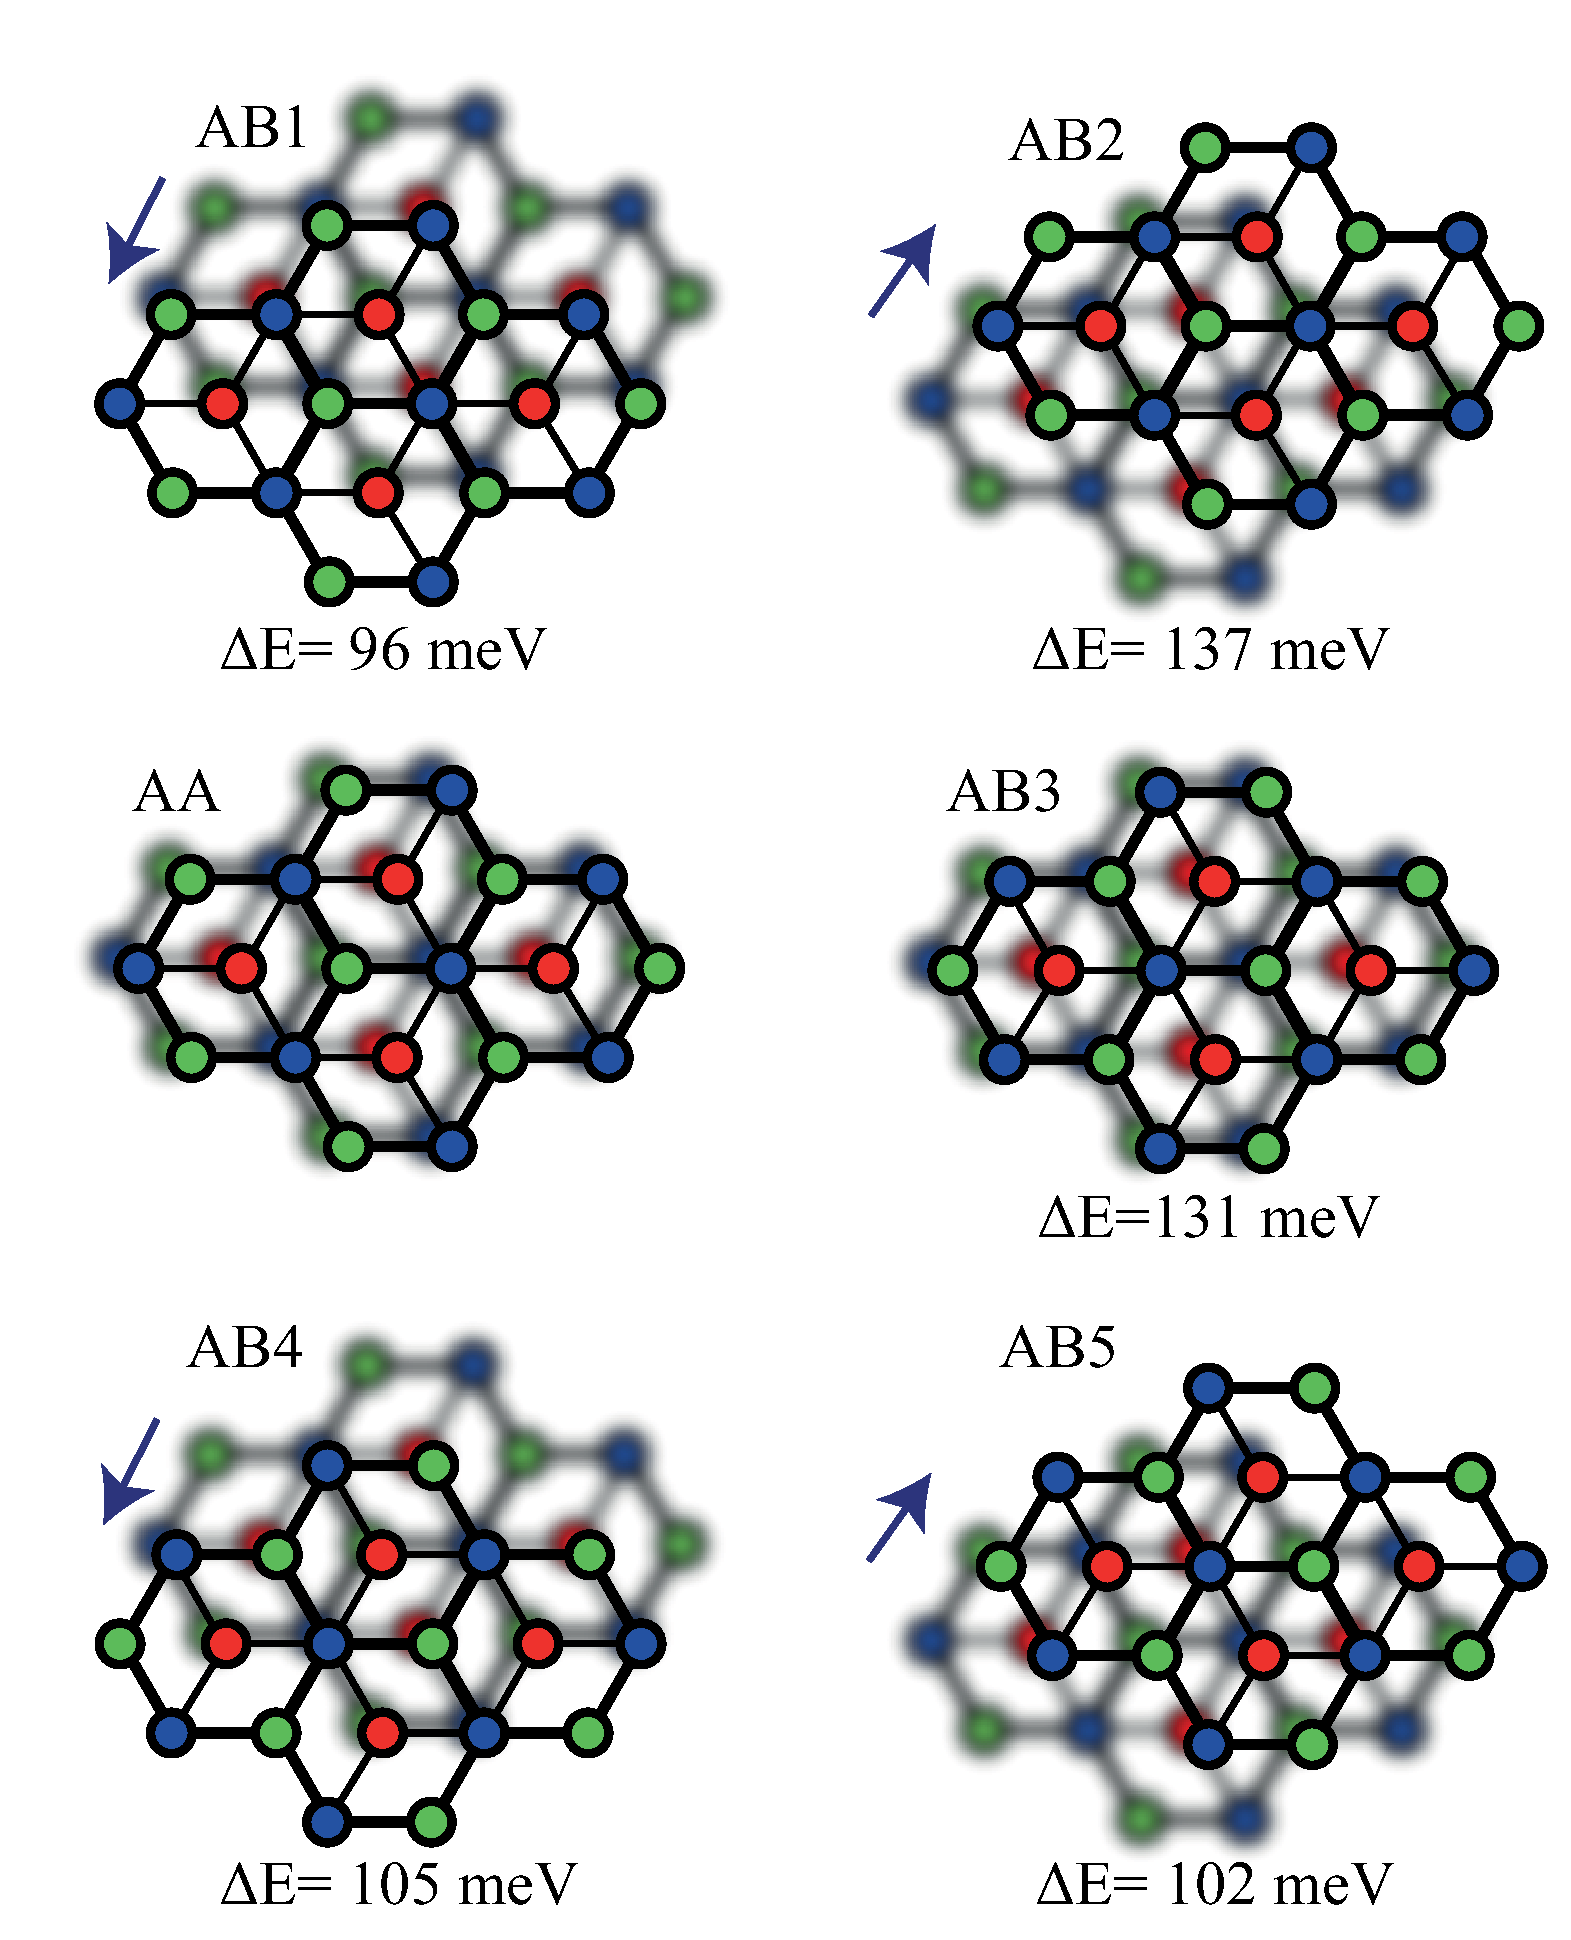
\includegraphics[width=0.7\textwidth]{stack_caoh2.eps}
\caption{\label{fig:stack_caoh2} Different stacked bilayers (bottom layer is blurred)
and their energy difference with respect to the AA stacking of Ca(OH)$_2$, i.e.
$\Delta$E=E$_{\text{ABX}}$-E$_{\text{AA}}$, (X=1,2,...,5). Energies are given
per formula of Ca(OH)$_2$. Blue, green and red circles are for Ca atom, 
upper hydroxyl group and lower hydroxyl group, respectively. For clarity, the 
bottom layer is shifted slightly.}
\end{figure}

\begin{figure}[htbp]
\centering
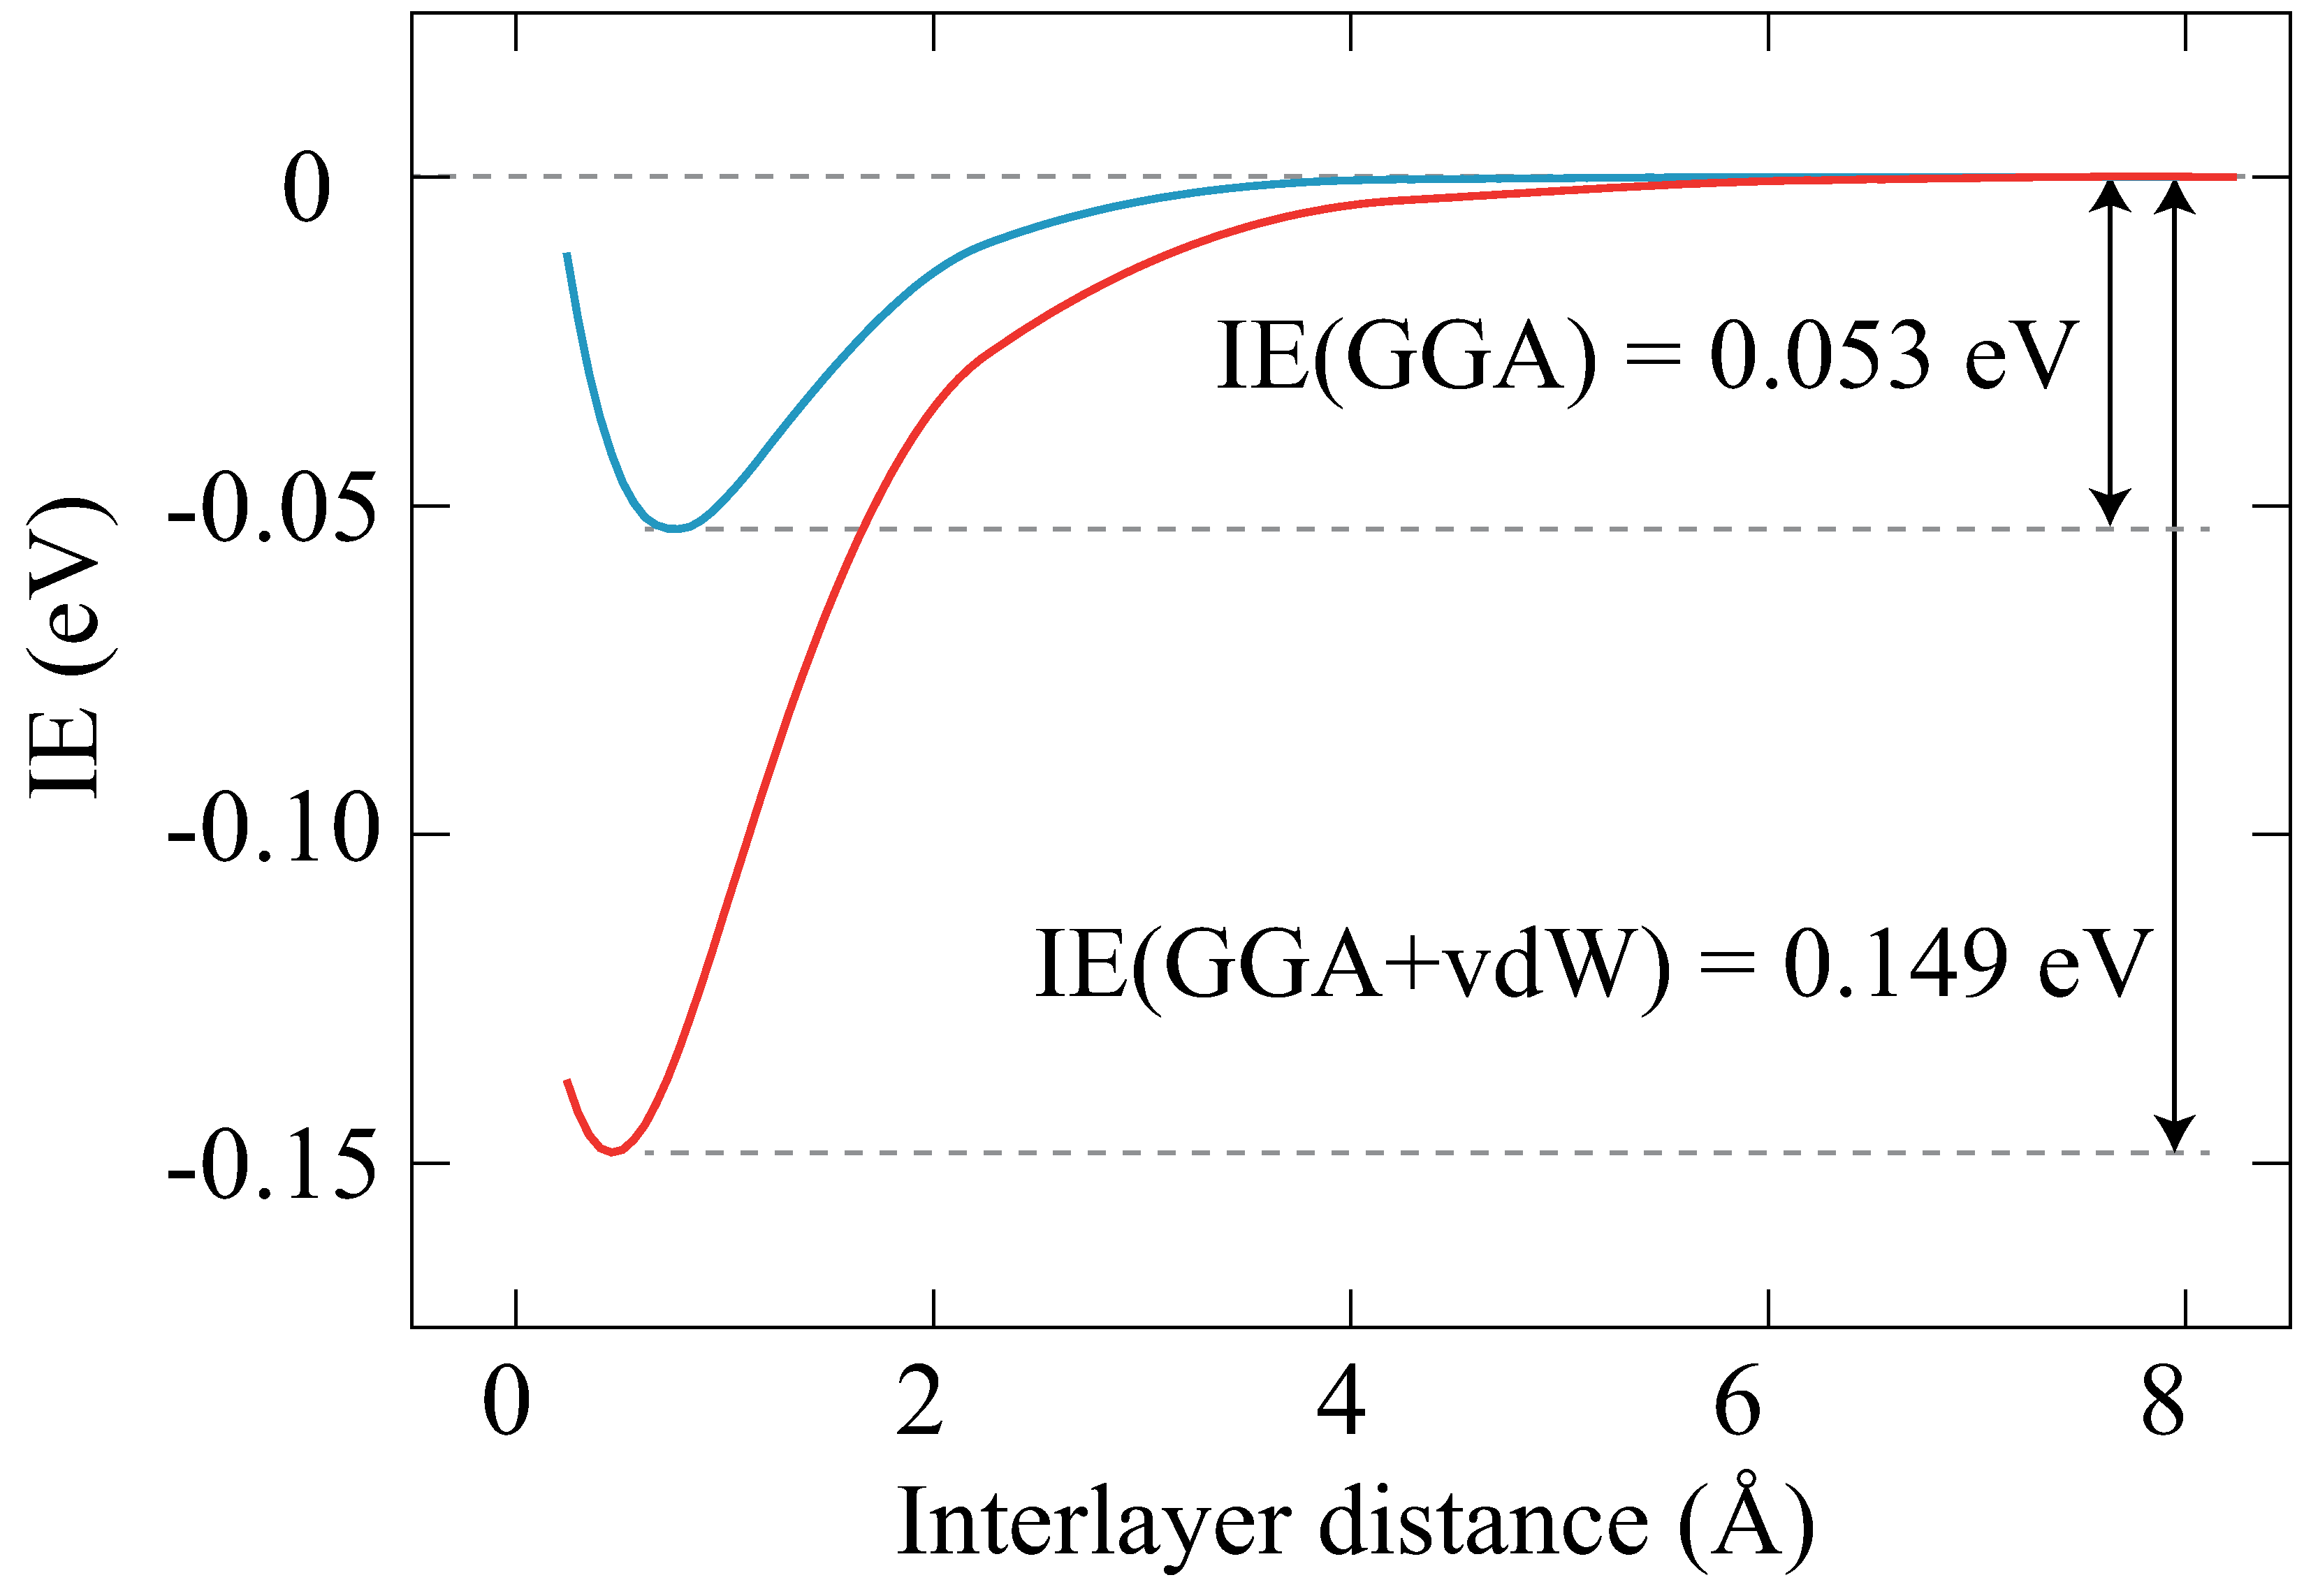
\includegraphics[width=0.7\textwidth]{int_caoh2.eps}
\caption{\label{fig:int_caoh2} Interlayer interaction energy per formula of
AA-stacked bilayer Ca(OH)$_2$. Blue and red curves are for GGA calculations
without and with vdW correction, respectively.}
\end{figure}

To investigate the nature of the interlayer interaction, we 
have calculated the interlayer interaction energy (IE) for the AA stacked 
bilayer structure of Ca(OH)$_2$. The IE is the energy difference between the 
total energy at a specific interlayer distance and that of a well
separated bilayer. The plot of IE versus interlayer distance is shown in Fig. 
\ref{fig:int_caoh2}, where the energy of the  well separated bilayer is defined as 
0 eV. Two sets of calculations were performed, one set only considers GGA 
exchange correlation; while another set considers both the GGA and vdW 
interaction. At the optimized interlayer distance for the bilayer structure, 
almost 2/3 of the attractive interaction comes from the van der Waals 
interaction, and this is consist with \citet{DArco1993} . They stated that
interlayer interaction of Brucite, one of the isomorphous of Portlandite, is
mainly a dispersion-type interaction. The nature of interlayer interaction in Ca(OH)$_2$ is mainly vdW type weak interaction. Our GGA+vdW calculations revealed that the interlayer interaction between two layers of Ca(OH)$_2$ (149 meV per formula) is much stronger than that of bilayers of MoS$_2$ (76 meV per formula).


\subsubsection{Electronic properties}\label{sec:electronic}


Our Bader charge transfer analysis showed that the final (initial) electron 
charge on Ca, O and H atoms after (before) the formation of the crystal are 
6.4$e$ (8.0$e$), 7.4$e$ (6.0$e$) and 0.4$e$ (1.0$e$), respectively. Therefore, 
in the bulk structure of Ca(OH)$_2$, Ca-O bonds, which are 
mostly in ionic character, are formed through 0.8$e$ charge transfer 
from each Ca to O atom.  Charge transfer is kept unchanged when it comes to the monolayer structure, except for the rest charge on H atom is 0.6$e$ in monolayer.


Our calculations on the electronic structure reveal that bulk Ca(OH)$_2$ is 
an insulator with a 4.37 eV direct band gap. As shown in \autoref{fig:elec_caoh2} (a), the valence band maximum (VBM) and the conduction 
band minimum (CBM) are located at the $\Gamma$ point. The partial density of 
states (DOS) shown in \autoref{fig:str_caoh2} (b) indicates that the major 
contribution to the states at the valence and conduction band edge originates 
from the O atoms, while deeper in the conduction band, states are mainly composed 
of the orbitals of Ca. The orbital character of a state at a particular band can 
also be deduced from a band and $k$-point decomposed charge density. As seen 
from \autoref{fig:elec_caoh2} (c), edges in the top of VBM have O-$p_x$ 
and O-$p_y$ orbital character, and the hybridization of these states are also 
shown in the same figure. While the CBM has some $p_z$ orbital 
character from the O atoms, but as the energy of the state increases, the $d$ 
orbitals from Ca atom start to contribute, see \circled{8} in the same figure.


Electronic properties of Ca(OH)$_2$ are quite different from similar
two-dimensional graphene-like structures. Unlike TMDs (such as MoS$_2$ and
WSe$_2$) that exhibit indirect-to-direct band gap crossover when going
from bulk to a single layer structure, Ca(OH)$_2$ is a direct band gap
semiconductor which is independent of the number of layers. Although the energy band gap
at the $\Gamma$ point decreases from 4.03 to 3.67 eV for a monolayer structure,
electronic dispersion of the valence band edge remains almost unchanged, see
\autoref{fig:elec_caoh2} (d). As shown in \autoref{fig:elec_caoh2} (e)  
the conduction states mainly originate from Ca atoms, while the valence states 
are mainly composed of the orbitals of O atoms. 

Our magnetic state analysis shows that unless a defect is formed in/on the 
structure, there is no spin polarization in the ground state of both bulk and monolayer Ca(OH)$_2$. Therefore, Ca(OH)$_2$ is a non-magnetic insulator regardless of its dimension for the structure. 

Moreover, it was seen that the spin-orbit interaction has no 
considerable effect on the bond lengths and the overall electronic dispersion 
(except for a 26 meV splitting in the VBM at the 
$\Gamma$ point, see \autoref{fig:elec_caoh2} (f)). Due to the presence of inversion symmetry of Ca(OH)$_2$, the 
degeneracy of spin-up and spin-down states still remains, this is also confirmed 
by the results of our calculation.


\begin{figure}[htbp]
\centering
\includegraphics[width=0.7\textwidth]{elec_caoh2.eps}
\caption{\label{fig:elec_caoh2} (a) and (d) are the Band structures, 
(b) and (e) are the partial DOS and (c) and (g) are the band and $k$-point decomposed charge densities of the bulk (c) and monolayer (g) Ca(OH)$_2$, respectively. The charge density are the band edges indicated in (a) and (d), isovalues are kept constant. (f) Band structure around $\Gamma$ point is shown with (dashed line) and without (solid line) spin orbit coupling. }
\end{figure}

\begin{figure}[htbp]
\centering
\includegraphics[width=0.8\textwidth]{suf_caoh2.eps}
\caption{\label{fig:suf_caoh2} Two lowest conduction band charge density of 
monolayer and bilayer Ca(OH)$_2$ at the $\Gamma$ point.}
\end{figure}

Band and $k$-point decomposed charge density in \autoref{fig:elec_caoh2} are 
kept with the same isosurface level for comparison. However, as we further 
reduced the isosurface level at \circled{4} in (d) and (g) of \autoref{fig:elec_caoh2}, which is the lowest conduction band of the 
monolayer at the $\Gamma$ point: $E_{c1}^{~\Gamma}$, charge density forms a planar 
state parallel to the layer on both sides, see \autoref{fig:suf_caoh2} (a), this
is also the case for the second lowest non-spin-resolved conduction band at the same
$k$-point: $E_{c2}^{~\Gamma}$, see \autoref{fig:suf_caoh2} (b). These two states are 
important due to their unique character and having energy right below ionization energy. Such exceptional states 
having free-electron-like dispersion were reported before\cite{Posternak1,Posternak2} for 
doped graphite. To study the trend in these states, the same states were plotted 
for bilayer Ca(OH)$_2$, see (c) and (d) in \autoref{fig:suf_caoh2}. $E_{c1}^{~\Gamma}$ and $E_{c2}^{~\Gamma}$ have lower energies than ionization energy. Therefore, electrons are still close and bond to both sides of monolayers as seen from charge density. In the case of bilayer, interestingly, these states appear only on one side of bilayer.

\subsubsection{Mechanical properties}

We present the quantities that describe the mechanical 
properties of Ca(OH)$_2$ in \autoref{tab:str2_caoh2}. 
At first, the in-plane Young's modulus of the bulk structure is calculated. 
Bulk Ca(OH)$_2$ has a in-plane Young's modulus (55.0 N/m) and in-plane shear 
modulus (21.23 N/m). Both these quantities indicating flexible nature to in-plane 
tensile and shear deformation of bulk Ca(OH)$_2$. In addition, bulk Ca(OH)$_2$ has 
an in-plane Poisson's ratio of 0.30.  Additionally, the value of the in-plane 
stiffness for bulk Ca(OH)$_{2}$ is calculated to be 60.1 J/m$^{2}$. 

If we go from bulk to bilayer Ca(OH)$_2$, we see a reduction in either the
in-plane Young's modulus or the in-plane shear modulus, which are 50.7 N/m and 
19.16 N/m, respectively. The in-plane Poisson's ratio on the other hand is 
slightly increased to 0.32 and become more spongy-like as opposite to more 
cork-like character\cite{poisson}. In addition, the in-plane stiffness value of 
bilayer Ca(OH)$_{2}$ is calculated to be 55.6 J$/$m$^{2}$. 

We found that monolayer Ca(OH)$_2$ has a quite low in-plane Young's modulus 
(50.7 N/m) when compared to BN (278.2 N/m). The in-plane Poisson ratio (0.33) 
and the in-plane shear modulus (19.08 N/m) of the monolayer are similar with 
those for bilayer, and for BN, they are 0.22 and 113.5 N/m respectively. The 
calculated values of the in-plane stiffness of monolayer Ca(OH)$_{2}$ is 53.2 
J$/$m$^{2}$. 

\subsubsection{Vibrational properties}\label{stability}
\begin{figure}[htbp]
\centering
\includegraphics[width=0.7\textwidth]{vib_caoh2.eps}
\caption{\label{fig:vib_caoh2} Phonon dispersion of monolayer Ca(OH)$_2$.}
\end{figure}

Lastly, for the analysis of the vibrational spectrum and further examination of 
the dynamical stability of monolayer Ca(OH)$_2$, we performed a 
calculation of the phonon spectrum using both the first-principles small 
displacement methodology (SDM)\cite{alfe} and density functional perturbation 
methodology (DFPT)\cite{baroni}. Here the non-quadratic dispersion of the 
flexural mode around the zone center is directly related to the insufficient 
FFT grid along the vacuum direction. It is seen from \autoref{fig:vib_caoh2} that 
similar to the Raman shift measurements observed from the bulk crystal 
structure, monolayer material has also high-frequency OH stretching 
modes at 3700-3800 cm$^{-1}$. 

Further analysis of the analysis of phonon 
branches shows that the decomposition of the vibration representation of optical 
modes at the zone center is $\Gamma = 4E_{u} + 2A_{2u} + 4E_{g} + 2A_{1g}$. As 
shown in right panel of \autoref{fig:vib_caoh2} there are four Raman-active phonon 
branches around 240, 350, 390 and 3700-3800 cm$^{-1}$. It is also worth to note 
that differing from other TMD structures having 1T phase, presence of H atoms 
results in existence of two different $E_{g}$ and $A_{1g}$ modes. Here the 
phonon dispersion having real eigenfrequencies in the whole Brillouin Zone, 
which is another indication of the stability of monolayer Ca(OH)$_2$.

\subsubsection{summary }\label{disc}

By performing first principle calculations on bulk, bilayer and 
monolayer Ca(OH)$_2$ and experimental confirmation of the bulk crystal 
layered structure, we have predicted several important properties of this 
material and their stability. We found that: (i) Ca(OH)$_2$ crystals are 
environmentally stable and their stable structures can be synthesized by 
experimental methods; (ii) Experimentally, we also demonstrated that Ca(OH)$_2$ 
crystals can be grown in layered form and also be exfoliated on arbitrary 
substrates; (iii) The dimensionality of Ca(OH)$_2$ will not change the 
electronic, structural and magnetic properties qualitatively, nevertheless 
intrinsic mechanical stiffness of each layer will become slightly stiffer as 
the system go from monolayer to bilayer. (iv) Interlayer interaction is mainly 
van der Waals dispersion-type force, and
the strength of the interaction is stronger than that of similar layered
materials (e.g MoS$_2$ and graphite). (v) The 
conduction states which have a free-electron-like character may be utilized for 
high-mobility electron transfer. 

We believe that the stable structure and the unique electronic properties of ultra-thin 
Ca(OH)$_2$, predicted for the first time here, will trigger interest in this 
new class of materials. 

\subsection[Few-layer of pentasilicene]{Few-layer of pentasilicene \footcite[This work is published in:][]{Aierken2016.pentasilicene}}

\subsubsection{Introduction\label{intro}}

Recently, a new 2D structure for carbon was proposed, called penta-graphene\cite{Zhang2015}. This crystal is composed entirely of pentagonal rings of C atoms with mixed sp$^2$/sp$^3$ orbital hybridization.  However, the silicon counterpart of this structure, penta-silicene, contains a dynamical instability in its monolayer form. A few attempts have been made to stabilize this new Si structure by hydrogenation\cite{Ding2015} and chemical doping\cite{Li2015b}. 

In the present work, we construct multilayer structures of penta-silicene. We use density functional theory to explore their stability and physical properties. Two types of stacking for the penta-silicene layers are found to give stable few-layer structures. These different stacking types lead to completely different electronic properties since one leads to metallic and the other to semiconducting behavior. Somewhat surprisingly, we found that bilayer penta-silicene has lower formation energy than the most stable hexagonal silicene bilayers. Furthermore, we found that the band gaps of these semiconducting penta-silicene bilayers can be tuned by mechanical strain. We first explore the stability of monolayer penta-silicene and demonstrate its dynamical instability. This forms the motivation to study few-layer systems. Then we investigate different stacking possibilities and the resulting stability. Further, we study their mechanical properties by calculating their elastic constants.  We also compare bilayer penta-silicene to the most stable bilayer hexagonal silicene structures. Lastly, The electronic properties of multilayered penta-silicene are discussed.

\subsubsection{Computational details}

\begin{footnotesize}
\begin{description}
\item[Simulation program:] VASP and Phonopy
\item[Energy cut-off:] 500 eV
\item[Pseudopotentials:] PBE-GGA(PAW)
\item[k points (Monkhorst-Pack):] 17$\times$17$\times$1 and 23$\times$23$\times$1 for insulating and metallic systems, respectively 
\item[Vacuum:] 20~\AA
\item[Energy and force convergence criterion:] 10$^{-8}$ eV and 10$^{-7}$ eV/\AA, respectively
\item[phonon calculation:] finite displacement method
\item[Supercell for phonon calculation:] $4\times4\times1$ and $3\times3\times2$ for few-layer and bulk systems, respectively
\item[\textit{Ab initio} molecular dynamics:] Parrinello-Rahman (NpT) dynamics \cite{vasp_npt1,vasp_npt2} and a Langevin thermostat \cite{vasp_Lgv}
\item[\textit{Ab initio} molecular dynamics (Energy cut-off):] 300 eV
\item[\textit{Ab initio} molecular dynamics (time step):] 2 fs
\item[\textit{Ab initio} molecular dynamics (temperature):] 100 K
\item[\textit{Ab initio} molecular dynamics (simulation time):] 6 ps
\end{description}
\end{footnotesize}

\subsubsection{Monolayer pentasilicene}\label{mono}

\begin{figure}[htbp]
\centering
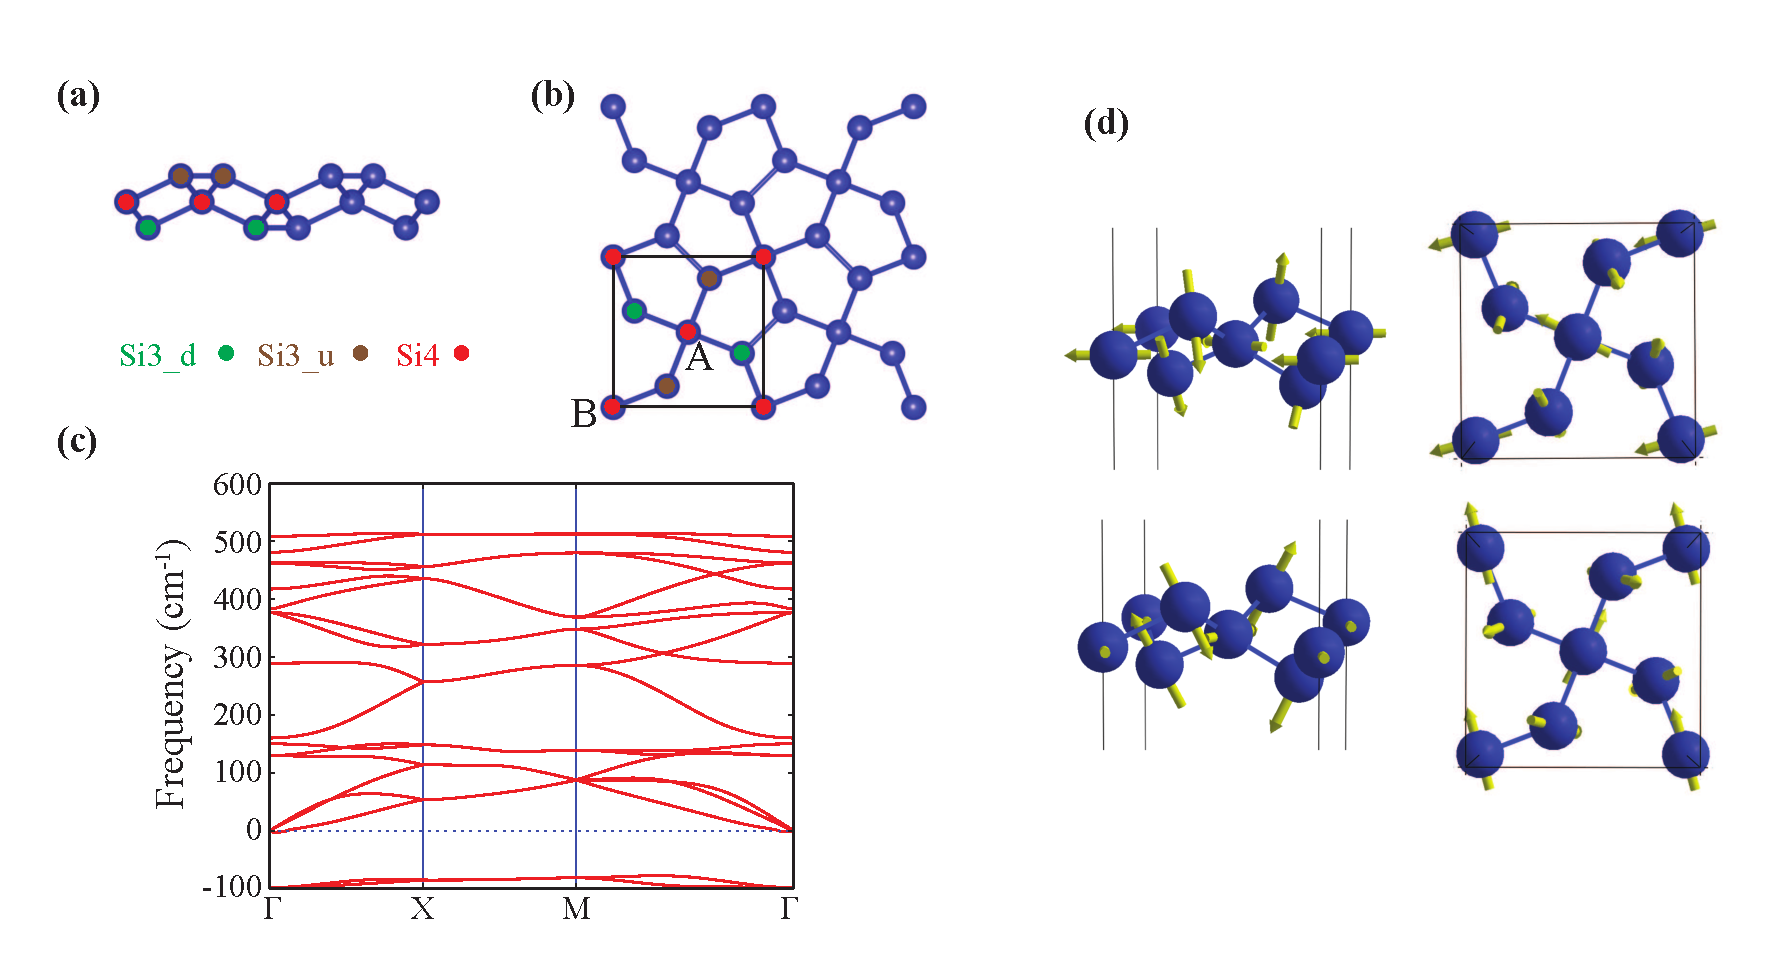
\includegraphics[width=\linewidth]{ps_monolayer.eps}%
\caption{(a) Side view and (b) top view of the atomic structure, (c) phonon spectrum and (d) two vibration modes with imaginary frequency of monolayer penta-silicene. Visualization of vibration modes is done with the V\_Sim package \cite{VSim}. \label{fig:ps_monolayer}}
\end{figure}

The layer group symmetry of monolayer penta-silicene (p-Si) is p$\overline{4}$2$_1$m (58). As shown in \autoref{fig:ps_monolayer}(a) and \autoref{fig:ps_monolayer}(b), the primitive cell contains six silicon atoms, of which two have fourfold coordination (Si4) and four have threefold coordination (Si3). Two of the Si3 atoms reside above the Si4 atoms, denoted as Si3\_u, while the other two are below the Si4 atoms, denoted as Si3\_d. The Si4 atoms are bonded to four Si3 atoms while the Si3 atoms are connected to two Si4 atoms and one neighboring Si3 atom. Note that the two Si4 atoms have equivalent environments which are rotated by approximately 41$^{\circ}$ with respect to each other. Therefore, in analogy to graphene, we can relate these two equivalent Si4 atoms to sublattices which in the following will be referred to as the A and B sublattice.

The dynamical stability of this structure can be studied through its phonon spectrum. As noted before\cite{Ding2015,Li2015b} the phonon spectrum of monolayer p-Si contains imaginary frequencies as shown in \autoref{fig:ps_monolayer}(c), which is a clear signature of its instability. The corresponding atomic vibrations of the two imaginary frequencies at the $\Gamma$ point are shown in \autoref{fig:ps_monolayer}(d). These modes correspond mainly to out-of-plane vibrations of the Si3 atoms with respect to the Si4 atoms. As a consequence, the structure is found to fall apart, indicating that there is no stable form of monolayer p-Si. However, the addition of extra layers could reduce these out of plane vibrations and stabilize the structure. This is the motivation to study few-layer p-Si.


\subsubsection{Multilayers of pentasilicene structures}\label{fews}

\begin{figure}[htbp]
\centering
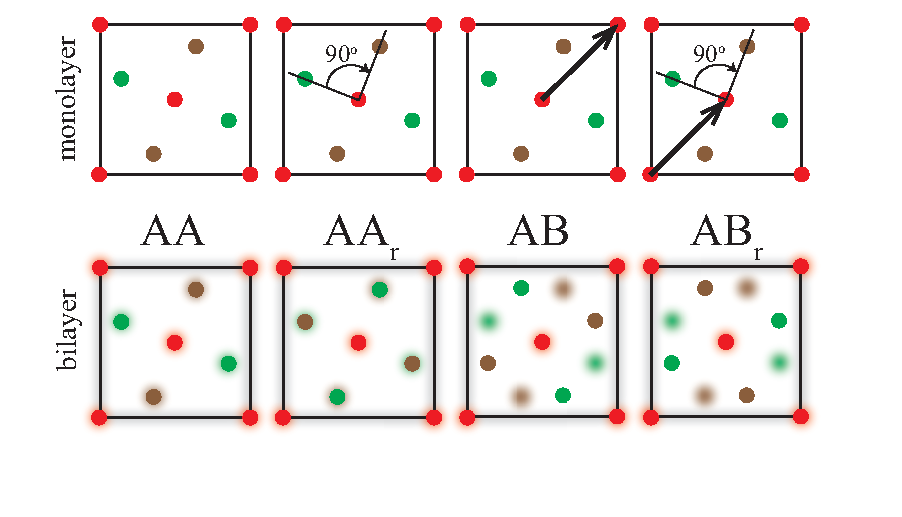
\includegraphics[width=0.8\linewidth]{ps_stackings.eps}%
\caption{ Schematic illustration of the four stacking types for bilayer p-Si. The colors of the symbols correspond to those of the monolayer in \autoref{fig:ps_monolayer}(a) and \autoref{fig:ps_monolayer}(b). The bottom layer in the bilayer is blurred for clarity. The arrow represents translation and the angle represents the rotation of the top layer with respect to the bottom layer. \label{fig:ps_stackings}}
\end{figure}

\begin{table}[htbp]
\centering
\caption{The cohesive energy (E$_{\text{coh}}$), the interlayer binding distance (d$_{\text{inter}}$), the interlayer binding energy (E$_{\text{inter}}$), number of interlayer bonds (N$_b$) and energy per bond (E$_{\text{bond}}$) of the four possible stacking types of bilayer p-Si. The interlayer binding energy per unit cell is defined as $E_{\text{inter}}=E_{\text{bi}}-2E_{\text{mono}}$. \label{bilayer_table}}
\begin{tabularx}{\textwidth}{@{\extracolsep{\fill}}XXXXXX}
\hline
\multirow{2}{*}{structure}  & E$_{\text{coh}}$ & d$_{\text{inter}}$ & E$_{\text{inter}}$& N$_b$ & E$_{\text{bond}}$ \\ 
 & (eV/atom) & (\AA) & (eV) & - & (eV) \\ \hline
AA & -4.129 & 0.795   & -3.502  & 4 & -0.875 \\
~AA$_r$ & -4.113 & 2.379   & -3.318  & 2 & -1.659 \\
AB & -3.968 & 2.174   & -1.574  & 2 & -0.787 \\
~AB$_r$ & -4.147 & 1.893   & -3.725  & 2 & -1.862 \\
~AB$_r^d$ & -4.185 & 1.896   & -4.174  & 2 & -2.087 \\ 
\hline
\end{tabularx}
\end{table}

When considering two layers, different stacking configurations are possible. Here we focus on the so-called AA and AB stacking modes of the aforementioned sublattices (see \autoref{fig:ps_stackings}). The stacking in which both layers have the same in-plane orientation and the Si atoms are put right on top of each other is called AA stacking. AB stacking arises by shifting the A sublattice of one layer to the B sublattice of the other. This nomenclature was also used by \citet{Wang2015} for bilayer penta-graphene. Although penta-silicene has a tertragonal lattice symmetry, the highest proper rotational symmetry order is two. Therefore, there are also two different possible orientations of the upper layer with respect to the lower one:  One in which the two layers have the same orientation and another in which one layer is rotated over 90$^{\circ}$ with respect to the other one. We denote this last orientation with a subscript $r$ to show that it results from a 90$^{\circ}$ rotation, e.g. AA$_r$. Therefore, there are four possible stacking types for bilayer p-Si. Note that AB$_r$ stacking corresponds to the recently proposed bulk T12 phase for group IVA elements\cite{Zhisheng2012}. However, as discussed in more detail below, perfect AB$_r$ stacking is not stable in the case of multilayer penta-silicene.  A considerable distortion of the outer layers is required to stabilize AB$_r$ stacking. The distorted structure, which will be referred to as AB$_r^d$ in the following, is obtained by breaking the symmetry between the two Si3 atoms at each surface side in AB$_r$ multilayers. In this way, one of the two Si3 atoms acquires sp$^2$ hybridization and looses an electron to the other Si3 atom that has sp$^3$ hybridization.

\begin{figure}[ht]
  \centering
  \begin{subfigure}{0.9\linewidth}
    \captionsetup{singlelinecheck=true}
    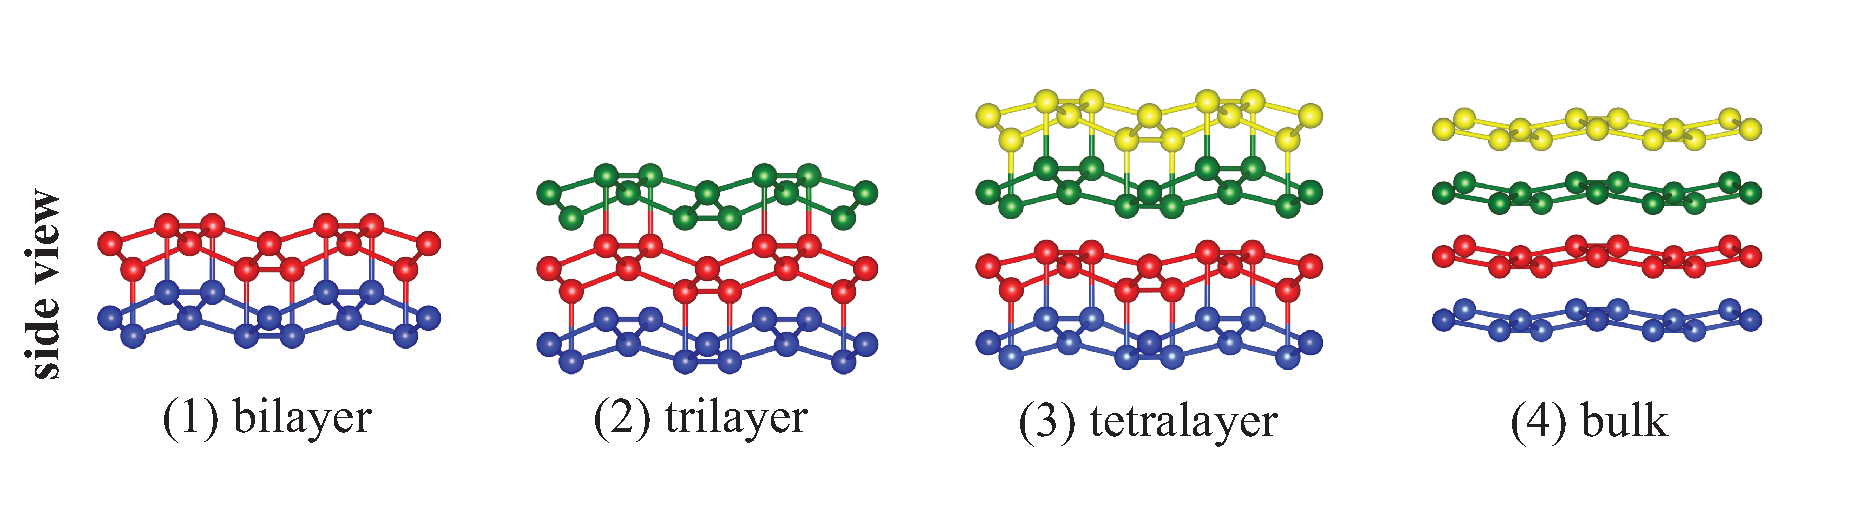
\includegraphics[width=\linewidth]{ps_AA_structures.eps}%   
    \caption{AA stacked structures \label{fig:ps_AA_structures}}
  \end{subfigure} 
  \begin{subfigure}{0.9\linewidth}
    \captionsetup{singlelinecheck=true}
    \includegraphics[width=\linewidth]{ps_AB_structures.eps}%
    \caption{AB$_r^d$ stacked few-layer and AB$_r$ stacked bulk structures \label{fig:ps_AB_structures}}
  \end{subfigure}
\caption{Atomic structure of the $2\times2$ supercell of few-layer p-Si. The number of atomic layers in the bulk structure is fixed to four for comparison (i.e.\ $2\times2\times4$ and $2\times2\times2$ supercells for AA and AB$_r$ stacked bulk p-Si). (Visualisation using VESTA \cite{vesta}). }
\end{figure}

In \autoref{bilayer_table}, we compare the energies of the different stacking modes. In all cases the Si4 atoms are not involved in interlayer bonding since their possible number of bonds is already saturated.  Except for the AA stacking where all Si3 atoms are bound to Si3 atoms from the other layer, only half of the Si3 atoms are bonded to the other layer in the other cases. In \autoref{bilayer_table}, the size of the interlayer binding energy and the strength per bond are given. The size of the bond energies indicate strong chemical bonding. The  AB$_r^d$ stacking mode clearly forms the most stable structure. For the rest of the paper, we will only focus on the most stable AA and AB-type stacking, i.e. AA and AB$_r^d$. 

\begin{landscape}

\begin{table}[htbp]
\centering
\begin{threeparttable}[b]
%\adjustbox{max width=\textwidth}{%
\caption{The layer (space) group for few-layer (bulk) systems. The lattice constant ($a$), the interlayer distance (d$_{\text{inter}}$), the nearest-neighbor bond length range (d$_{\text{min/max}}$), the cohesive energy (E$_{\text{coh}}$), and the band gap (PBE) of few-layer and bulk p-Si.}
\label{few-layer-table}
\begin{tabular}{cllccccccc}
\hline
stacking & structure & layer/space group & $a$ (\AA) & d$_{\text{inter}}$ (\AA) & d$_{\text{min}}$ (\AA) & d$_{\text{max}}$ (\AA) & E$_{\text{coh}}$ (eV/atom) & band gap (eV)   &  \\[3pt]  \hline
-& monolayer & p$\overline{4}$2$_1$m (58) & 5.587  & - & 2.233 & 2.363 & -3.837 &  0.046 (M$\rightarrow \Sigma$) & \\[3pt] \hline
\multirow{4}{*}{AA}
& bilayer    & \multirow{3}{*}{p$\overline{4}$2$_1$m (58)} & 5.907  & 0.795 & 2.363 & 2.468 & -4.129 & metal  &  \\[3pt]
& trilayer   &   &5.887   & 1.085    & 2.330 & 2.606 & -4.108           & metal          &  \\[3pt]
& tetralayer &   & 5.980  & 0.996/1.794\tnote{a}   & 2.368 &	2.478   & -4.150           & metal          &  \\[3pt]
& bulk       & P$\overline{4}$2$_1$m (113)  & 6.234  & 1.769    & 2.398 & 2.463          & -4.204            & metal           &  \\[3pt] \hline
\multirow{3}{*}{AB$_r^d$}                          
& bilayer   & pb2b (30) pm2a (31) & 5.222            & 1.896      &2.303 &	2.403         & -4.185           & 0.119 (M$\rightarrow \Sigma$) &  \\[3pt]
& trilayer  & p1 (1) & 5.222            & 1.989     & 2.298 &	2.413           & -4.291           & 0.247 (M$\rightarrow \Sigma$) &  \\[3pt]
& tetralayer & pb2b (30) pm2a (31) & 5.221            & 1.997       & 2.298	 & 2.413         & -4.345           & 0.232 (M$\rightarrow \Sigma$) &  \\[3pt]
AB$_r$ & bulk      & P4$_2$/ncm(138) & 5.220         & 1.999       & 2.358 &	2.413         & -4.508           & 1.329 (M$\rightarrow \Delta$) & \\ \hline
\end{tabular}
\begin{tablenotes}
\item [a]The first and the second number indicate the interlayer distance between two monolayers and two bilayers, respectively.
\end{tablenotes}
\end{threeparttable}
\end{table}

\end{landscape}

We also investigated the stability of trilayer, tetralayer and bulk p-Si structures by adding extra layers to the stable bilayers mentioned above, their structures are shown in \autoref{fig:ps_AA_structures} and \autoref{fig:ps_AB_structures}. We list their structural and energetic properties in \autoref{few-layer-table}. Extra layers increase the cohesive energy per atom due to a smaller ratio of surface atoms. For AA stacking, adding a 4th layer to a trilayer system results in a double bilayer system with lesser bonding between them. Going to AA bulk, the interlayer interaction appears to be further reduced and the buckled layers become more flat. Adding extra layers to an AB$_r^d$ bilayer results in similar structures in which the Si3 atoms of the surface layers become distorted. For bulk, the undistorted AB$_r$ structure is found in which $\overline{4}$-fold symmetry is restored.



\subsubsection{Stabilities}\label{stab}

\begin{figure}[htb]
\centering
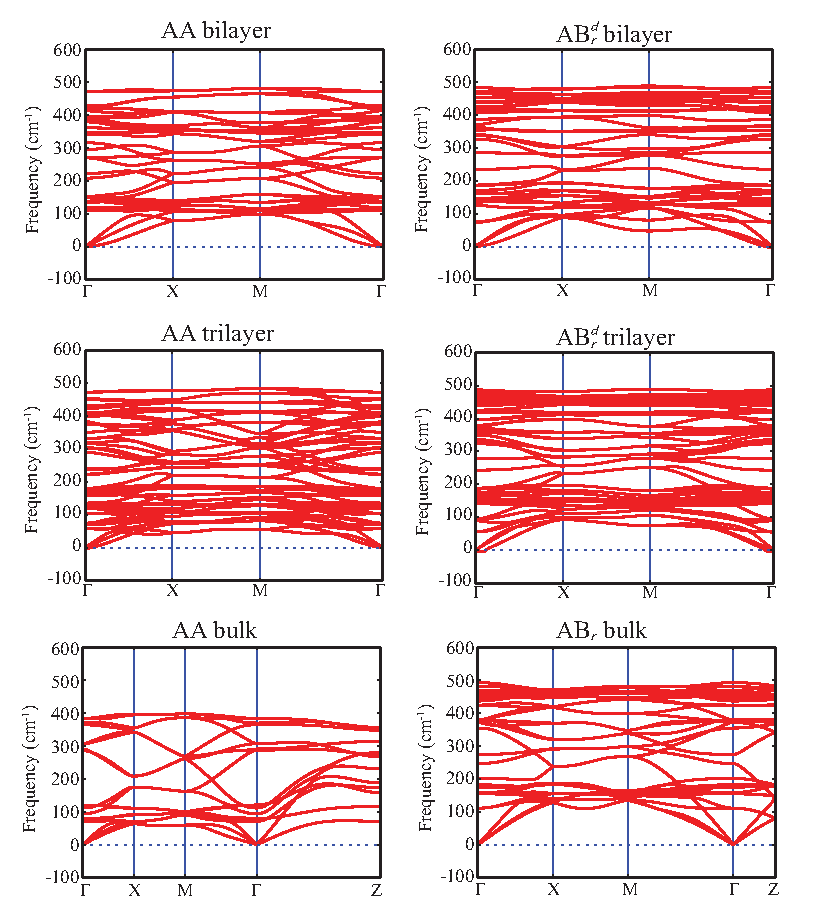
\includegraphics[width=0.9\linewidth]{ps_phonon_spectrum.eps}%
\caption{Phonon spectra of different-stacked few-layer p-Si. \label{fig:ps_phonon}}
\end{figure}

In this section we investigate the stability of the different multilayer structures discussed above.
Phonon calculations for the AA and AB$_r$ stacking modes reveal that only the AA bilayer is dynamically stable at low temperature. The extra bonds of the Si3 atoms in AA-stacked structures effectively reduce out-of-plane vibrations and stabilize the structure. Although the AA-stacked bulk structure has weaker interlayer bonding, its phonon spectrum contains no imaginary frequencies, indicating its dynamical stability. The AB$_r$-stacked layers, on the other hand, exhibit similar out-of-plane vibrations of the outermost Si atoms as a monolayer. For AB$_r^d$-stacking the distortion of the outermost layer removes the instabilities from the phonon spectrum, so that these structures are also dynamically stable. 

It is also interesting to see whether these structures remain stable at finite temperature. To this end, we performed \textit{ab initio} molecular dynamics calculations at a temperature of 100 K. The evolution of the cohesive energy as a function of simulation time is shown in \autoref{fig:ps_MD}. For comparison, the results for the dynamically unstable monolayer are also shown. The monolayer laterally shrinks and becomes a disordered multilayered system. The AA and AB$_r^d$ bilayer systems, on the other hand, remain stable and retain their crystalline structure.

\begin{figure}[htbp]
\centering
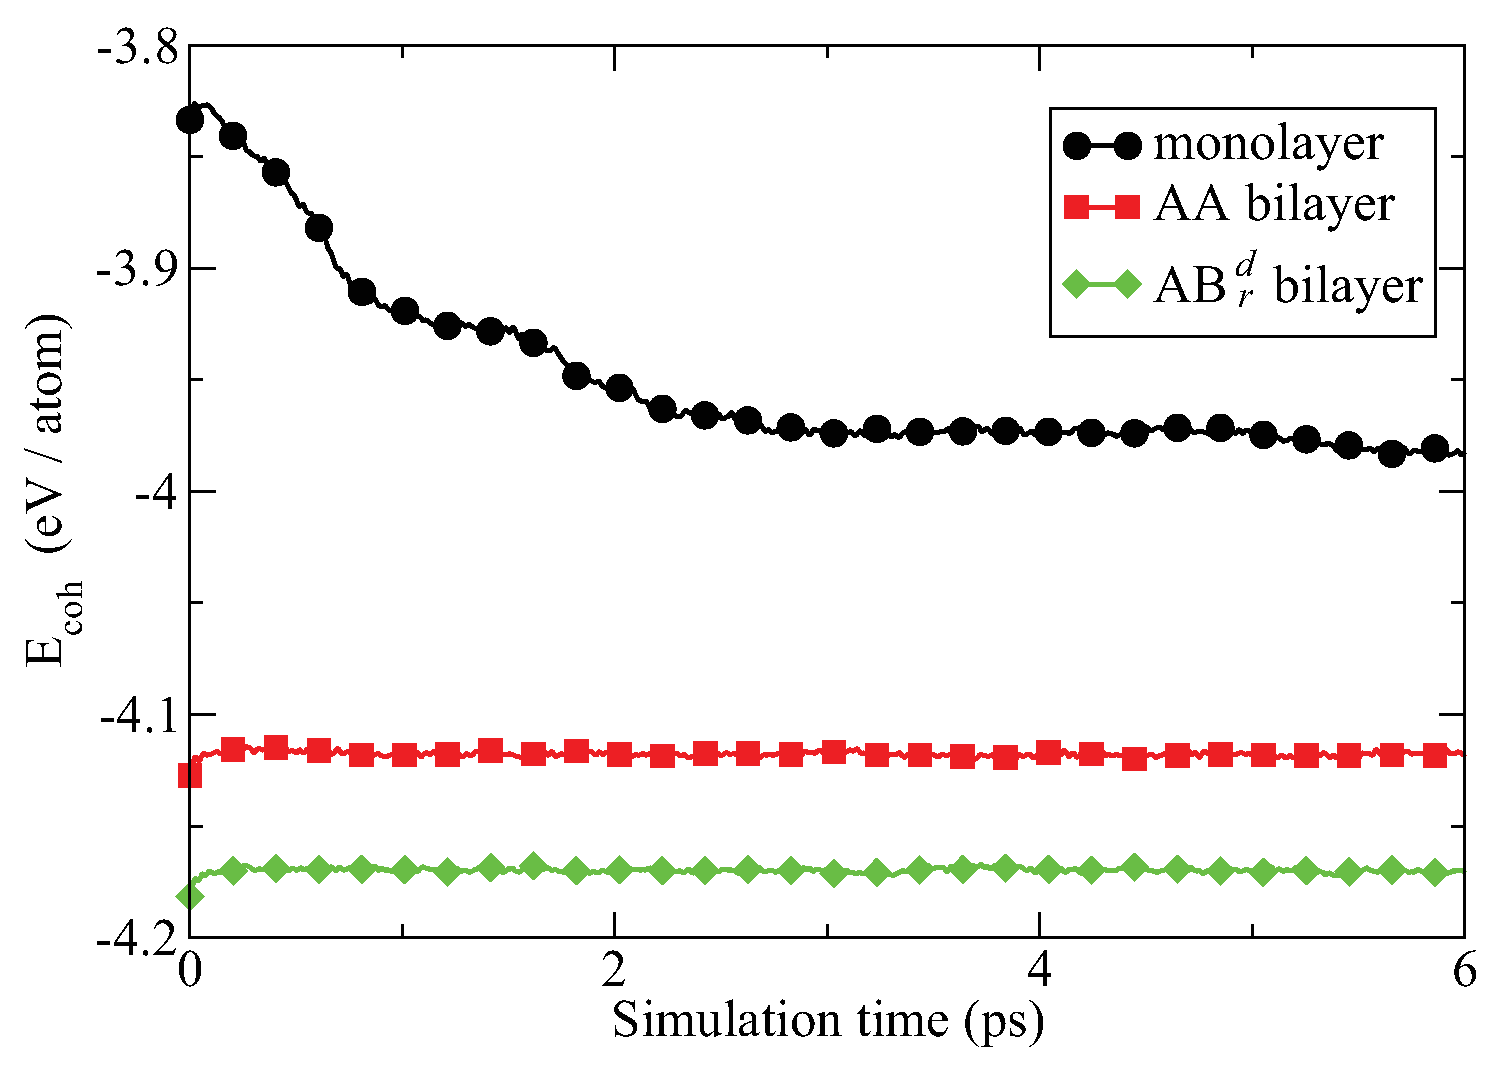
\includegraphics[width=0.7\linewidth]{ps_ab_initio_MD_100K.eps}%
\caption{The cohesive energy of monolayer and AA and AB$_r^d$ stacked bilayer p-Si as a function of time at a temperature of 100 K under NpT-ensemble. \label{fig:ps_MD}}
\end{figure}

As a final stability check, we investigate the mechanical stability of bilayer p-Si which is determined by the elastic constants of the structures. If the elastic constants satisfy the necessary and sufficient Born criteria generalized by \citet{Mouhat2014}, the structures are mechanically stable. AA bilayer p-Si belong to the layer group symmetry of p$\overline{4}$2$_1$m, which belongs to the tetragonal symmetry groups, and the independent elastic constants in 2D are: $C_{11}$= 101.43 N/m, $C_{12}$= 36.36 N/m and $C_{66}$ = 39.53  N/m. In the case of AB$_r^d$ bilayer p-Si, the crystal possesses pb2b or pm2a layer group symmetry which belongs to the orthorhombic crystal systems, and the independent elastic constants are: $C_{11}$=$C_{22}$= 63.83 N/m, $C_{12}$=26.92 N/m and $C_{66}$ = 50.43 N/m.  For mechanical stability, the following criteria must be fulfilled for 2D tetragonal systems:
\begin{equation}
C_{11}>|C_{12}|, C_{66}>0,
\end{equation}
while 2D orthorhombic systems should satisfy:
\begin{equation}
C_{11}>0,C_{11}C_{22}>C_{12}^2, C_{66}>0.
\end{equation}
As one can see, these criteria are satisfied by AA and AB$_r^d$ bilayer p-Si which ensures their mechanical stability. Additionally, in \autoref{mechanical}, we list the  (2D) Young's modulus, shear modulus and Poisson's ratio of bilayer p-Si systems. An interesting aspect of the possion's ratio of AB$_r^d$ is that it is quite high and close to the theoretical limit of 0.5. This means that this 2D material, prefers to change its shape rather than its surface area under strain, similar to the (3D) cases of rubber and water.

\begin{table}[htbp]
\centering
\caption{Mechanical properties of AB$_r^d$ bilayer p-Si}
\label{mechanical}
\begin{tabularx}{\textwidth}{lXXX}
\hline
Stacking & $E[N/m]$ & $G[N/m]$ & $\nu$ \\ \hline
AA & 88.40 & 39.53 & 0.36 \\ 
AB$_r^d$ & 52.47 & 50.41 & 0.42  \\ \hline
\end{tabularx}
\end{table}

\subsubsection{Relative phase stability}\label{hexa}

In this section we compare the cohesive energy of bilayer p-Si to the more familiar bilayer hexagonal silicene structures (h-Si).  We examined 3 different stacking types for h-Si bilayers, denoted as h-Si1, h-Si2, and h-Si3. To the best of our knowledge, these are the most stable hexagonal bilayer structures of silicene predicted so far. The h-Si2 structure corresponds to the re-DL-Si structure suggested by \citet{Morishita2011} and the h-Si3 is the hex-OR-2$\times$2 structure that was recently proposed by \citet{Sakai2015}. These structures are constructed from the structure information provided by the authors in the supplementary material of the corresponding papers and re-optimized with our computational procedure. The h-Si1 is a new stable bilayer h-Si structure that we discovered (see ESI\dag~for details). It is composed of two planar, non-buckled, compressed hexagonal silicene planes that are shifted along the crystal plane. This structure is interesting because although its cohesive energy is close to the former two cases, it has a non-buckled nature. To the best of our knowledge, it is the most stable non-buckled bilayer silicene discovered so far. 

The cohesive energies of all the stable bilayer Si systems are given in \autoref{h-Si_table}. It is seen that the AB$_r^d$ bilayer p-Si system has the lowest energy, about 10 meV/atom less than the most stable hexagonal silicene bilayer h-Si3.  This means that the AB$_r^d$ p-Si structure is the most stable bilayer silicon structure predicted so far, which is a very surprising result. The AA-stacked p-Si has slightly higher energy than h-Si2 and h-Si3.


\begin{figure}[htbp]
\centering
\includegraphics[width=0.8\linewidth]{ps_h-silicene.eps}%
\caption{Top and side views of the atomic structures of the 2 $\times$ 2 supercell of the three examined hexagonal silicene bilayers. \label{fig:ps_h-Si}}
\end{figure}

\begin{table}[htbp]
\centering
\caption{The interlayer distance d$_{\text{inter}}$, the nearest-neighbor bond length range (d$_{\text{min/max}}$) and the cohesive energy per atom E$_{\text{coh}}$ of the most stable hexagonal bilayer silicene and bilayer p-Si. }
\label{h-Si_table}
\begin{tabularx}{\linewidth}{lXXXX}
\hline
\multirow{2}{*}{structure}  &   d$_{\text{inter}}$ & d$_{\text{min}}$ & d$_{\text{max}}$ & E$_{\text{coh}}$  \\ 
 &   (\AA) & (\AA) & (\AA) &  (eV/atom) \\
 \hline
AA bilayer p-Si  &  0.795  & 2.363  & 2.468  & -4.129 \\
AB$_r^d$ bilayer p-Si  &  1.896  & 2.303  & 2.403  & -4.185 \\
h-Si1            &  2.175  & 2.358  & 2.418  & -4.115 \\
h-Si2            &  1.579  & 2.298  & 2.453  & -4.165 \\
h-Si3            &  1.378  & 2.288  & 2.473  & -4.175 \\ 
\hline
\end{tabularx}
\end{table}

\subsubsection{Electronic properties}\label{elec}

\begin{figure}[htbp]
\centering
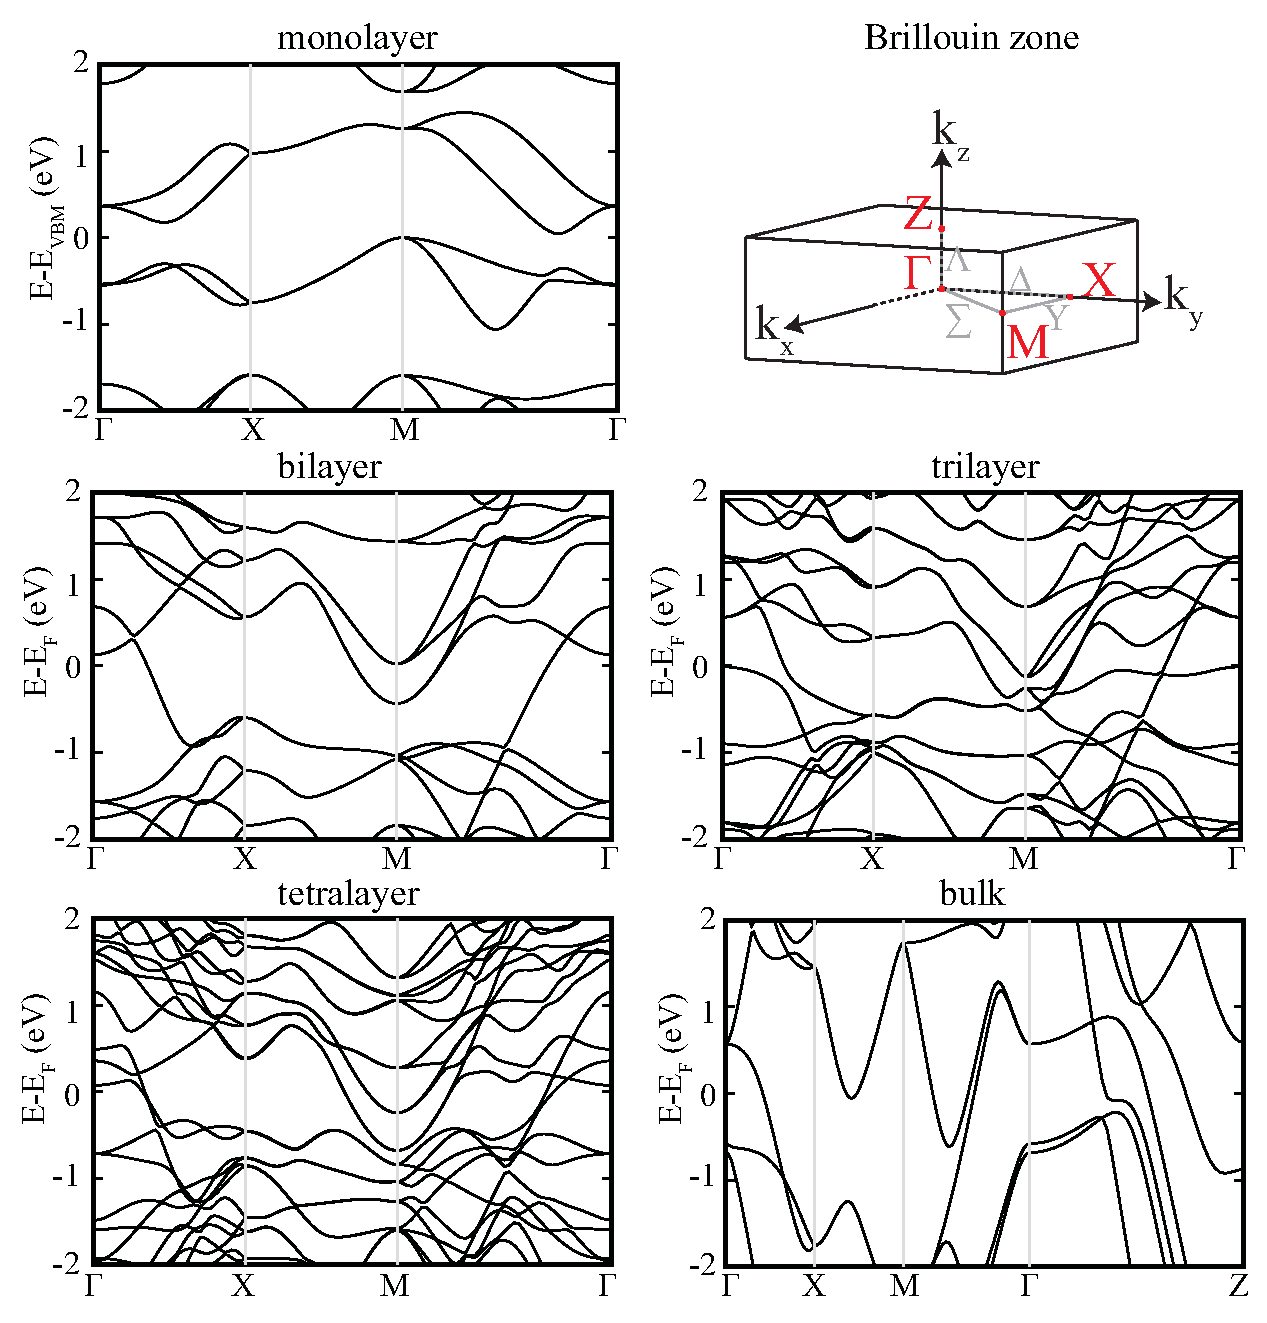
\includegraphics[width=0.7\linewidth]{ps_AA_bands.eps}%
\caption{Electronic band structure of AA stacked few-layer and bulk p-Si, and a schematic of the first Brillouin zone. \label{fig:AA_bands}}
\end{figure}

\begin{figure}[htbp]
\centering
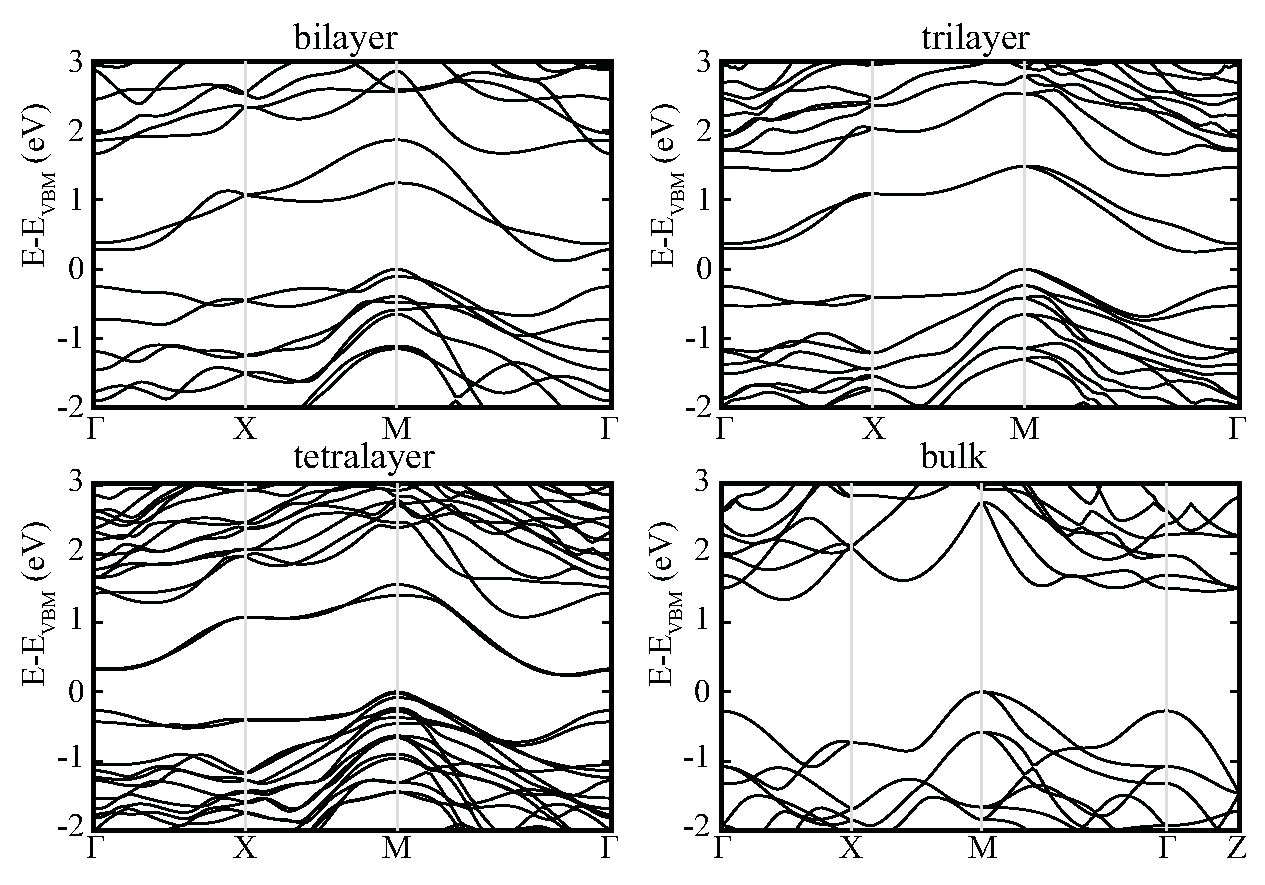
\includegraphics[width=0.7\linewidth]{ps_AB_bands.eps}% 
\caption{Electronic band structures of AB$_r^d$ stacked few-layer and AB$_r$ stacked bulk p-Si. The results for the monolayer are shown for comparison.\label{fig:AB_bands}}
\end{figure} 

\begin{figure}[htbp]
\centering
\includegraphics[width=0.7\linewidth]{ps_charge_density.eps}%
\caption{The charge distribution of CBM and VBM in AB$_r^d$ stacked few-layer and AB$_r$ stacked bulk p-Si. The results for the monolayer are shown for comparison.\label{fig:charge_density}}
\end{figure}

In the last part of this work, we investigate the electronic properties of few-layer and bulk p-Si. These electronic properties are mainly determined by the electronic spectrum. In \autoref{fig:AA_bands} and \autoref{fig:AB_bands}, the electronic band structure of respectively AA and AB$_r^d$ p-Si multilayers and their bulk counterpart is shown. The band structure of the unstable monolayer is also calculated for comparison. Monolayer p-Si is an indirect semiconductor with a band gap of 0.046 eV (PBE). The band-edge states are mainly composed of $p_z$ orbitals of Si3 atoms. In contrast to this, all AA-stacked multilayers are metallic. In the case of the AB$_r^d$ structure, the semiconducting properties of monolayer p-Si are preserved, but the band gap changes somewhat with the number of layers. This can be understood from the position of the electron and hole states which correspond to the conduction band minimum (CBM) and the valence band maximum (VBM), respectively. As seen in \autoref{fig:AB_bands}, the VBM and CBM states are always localized on the outermost layers. In other words, the electronic properties are mainly determined by the surface region which is nearly independent of the slab thickness. For AB$_r$-stacked bulk p-Si, there is no surface and the VBM and CBM correspond to bulk states. This explains the much larger band gap (1.33 eV) in the bulk case. 


\subsubsection{Summary\label{conc}}

In this work, we proposed several stable structures for few-layer pentasilicene. The stability of these structures was confirmed via their phonon spectrum, finite-temperature molecular dynamics, and their mechanical properties. The type of stacking mode, AA or AB, of few-layer pentasilicene has a crucial influence on the electronic properties: AA-stacked systems are metallic, while AB$_r^d$ stacked ones are semiconducting . Surprisingly, the AB$_r^d$ stacked bilayer pentasilicene has lower energy than the most stable bilayer hexagonal silicene structures, which makes it the most stable predicted form of bilayer silicon.  


\section{Mechanical strain}

\subsection[Carrier mobility enhancement in TiS$_3$ monolayer with strain]{Carrier mobility enhancement in TiS$_3$ monolayer with strain \footcite[This work is published in:][]{Aierken2016.mobility}}

\subsubsection{Introduction}

Recently, a number of two-dimensional (2D) crystal materials  beyond graphene \citep{Novoselov666,Novoselov26072005,Geim2007} have been synthesized or have been theoretically predicted to be stable. For example, transition metal dichalcogenides (TMDs) \cite{RadisavljevicB2011,Zeng2011,Ataca2012,Liu2015, tongay-res2, PhysRevB.89.155433}, phosphorene family \cite{p1,Han2014,Adam2015,Guan2014,deniz1,deniz3}, transition metal carbides/carbonitrides (Mxenes)\cite{ADMA:ADMA201304138}, and penta-graphene \cite{Zhang2015} have attracted a growing research interest.  Many of these materials have distinct properties with respect to their bulk counterpart, ranging from the nature of the band gap\cite{Mak2010} to the size of the thermal conductivity \cite{Alexander2008}.  For future electronic device applications, it is the high mobility and band gap of these materials, which has drawn significant attention of the researchers. Although graphene is a fascinating material due to e.g. its ultra high mobility, it has however one significant disadvantage, i.e. it lacks a band gap, and thus is unsuitable for digital electronic applications. This drawback has triggered  extensive efforts to search for new materials  having a finite band gap and high mobility. Recently synthesized phosphorene and monolayer TiS$_3$\cite{ADOM:ADOM201400043,ADMA:ADMA201405632} are examples of such promising materials for high-performance applications. On the other hand, the modification of physical and chemical properties through various methods, e.g. chemical functionalization, heterostructure and mechanical strain, could pave a path for the exploration of the hidden features which do not manifest themselves at the pristine structure. 

Enhancement of the mobility under strain has been reported and measured before for silicon layers on Si$_x$Ge$_{1-x}$ substrates \cite{Vogelsang1993,Welser1994}, according to which a mobility enhancement up to about 76 \% at room temperature was achieved. Recently, first-principles calculations have been frequently used to determine the intrinsic mobility of 2D materials.\cite{Kaasbjerg2012,Zhang2014,Yongqing2014}. There are also several works that investigated the mobility of monolayer materials under strain\cite{fei,Henry2015,Sheng2015}. 
%including strain-controlled anisotropic of mobility in phosphorene \cite{fei}, vertical compression of phosphorene bilayer leads to two orders of magnitude increment of mobility%\cite{Henry2015}, strain-enhanced mobility of MoS$_2$ up to a factor of 10 \cite{Sheng2015}. 
%In the last two cases, enhancement of mobility contribute from decrease of deformation potential constant which consist with our situation that will be discussed in our results. 
Inspired by significant improvements of the transport properties of 2D materials by the help of appropriate strain type and size, we investigate the strain dependence of  carrier mobility of TiS$_3$ monolayer under mechanical strain at 300 K. We find that more than an order of magnitude enhancement of the electron mobility can be achieved by the tensile strain. Furthermore the hole mobility also has moderate enhancement.


\subsubsection{Computational details}
We perform first-principles calculations in the framework of
density functional theory (DFT) as implemented in the Vienna
$ab$-$initio$ simulation package (VASP) \cite{VASP1,VASP2,VASP3,VASP4}. The projector augmented wave (PAW)
method is used to take into account the electron-ion interaction\cite{PAW1,PAW2}.
Since the calculated mobility are strongly sensitive to the accuracy of the calculation, we use a set of input parameters that promise to deliver highly accurate results.
Such crucial parameters are  700 eV energy cut-off for the plane wave basis set,  10$^{-8}$ eV for self-consistent total energy convergence,  10$^{-7}$ eV/{\AA} for the ionic step force convergence,  25$\times$25$\times$1 $k$-point mesh for the Brillouin zone sampling, and a large vacuum space of 20 {\AA} between periodic images along the \textit{c} direction that is perpendicular to the TiS$_3$ layer. Exchange-correlation interactions are treated with the generalized gradient approximation (GGA) within the Perdew-Burke-Ernzerhof (PBE) formulation \cite{GGA-PBE1,GGA-PBE2}.  Band gap is underestimated due to well-known semilocal functional band gap problem. However, for the position shifts of the valence and conduction band edges with an applied tensile strain, the semilocal functional can provide consistent results and trends when compared to hybrid functionals and has  been successfully used in  previous studies for the determination of the mobility in 2D material \cite{Meng-Qiu2009,Yongqing2014,fei}. Phonon calculations are performed in a supercell of 2$\times$3$\times$1 using the finite displacement method as implemented in VASP together with the PHONOPY program \cite{phonopya}. 

To determine the mobility of electron and  hole, we use the deformation potential theory together with the effective mass approximation \cite{Bardeen1950}, which has been previously applied to several 2D systems\cite{Xi2012,Qiao2014a,Dai2015,Kang2015}.
The mobility, $\mu$, of a 2D system is given by: 
\begin{equation} \label{equ}
\mu=\frac{2e\hbar^3C}{3k_BT|m^*|^2E_d^2}.
\end{equation}
where $e$ is the electron charge and $\hbar$ is the reduced planck constant. $C$ is the elastic modulus along the transport direction. It is defined as $C=(\partial^2E_{total}/\partial\varepsilon^2)/S_0$, where $E_{total}$ is the calculated total energy of TiS$_3$, $\varepsilon$ is the strain applied along the transport direction and $S_0$ is the equilibrium 2D area of the unit cell. $k_B$ is the Boltzmann constant. T is the temperature, which is equal to 300 K throughout the paper unless stated otherwise. $m^*$ is the effective mass of the carrier along the transport direction calculated from $1/m^*_{e(h)}=\partial^2E_{c(v)}(k)/\partial k^2\hbar^2$, where $E_{c(v)}(k)$ is the energy dispersion near the CBM (VBM). $E_d$ is the deformation potential constant (DPC) along the transport direction. It is defined as $E_d^{e(h)}=\Delta E_{CBM(VBM)}/(\delta l/l)$, where $\Delta E_{CBM(VBM)}$ is the energy shift of the band edges with respect to the vacuum level under a small dilation $\delta l$ of the lattice constant $l$. We fix $\delta l/l$ to 0.005 that is inspired from previous calculations \cite{Dai2015}. In this theory,  the dominant scattering process is the longitudinal acoustic phonon scattering (AS). However, for a polar material, scattering on  optical phonon modes and other scattering sources should be taken into account at high temperatures\cite{Kaasbjerg2012}. Nevertheless, in this work, we will focus solely to the effect of AS to mobility and its dependence on the strain for the following reasons: 1) The dominant role of AS is not suppressed in polar materials, so it is still an important part that determines the mobility, 2) To separately study different mobility-controlled mechanism, specially their strain dependence, and 3) Computationally less expensive. 


\subsubsection{Unstrained system}

\begin{figure}[htb]
\centering
\includegraphics[width=0.5\linewidth]{Mob_str.eps}
\caption{(a) Top and (b) tilted views of a 2$\times$2 supercell of monolayer TiS$_3$.  Two crystallographic directions (where the strain is applied or the mobility is calculated) are shown with red and green arrows. \label{structure} }
\end{figure}

%The atomic structure of TiS$_3$ monolayer is shown in Fig.~\ref{structure}. The unit cell has a monoclinic crystal structure. The calculated lattice constants  are \textit{a} =  5.03 ~{\AA} and \textit{b} = 3.41~{\AA}, in good agreement with previous calculations \cite{Kang2015,Jin2015} and close to the experimental values for the bulk structure ($a$=4.958, $b$=3.401)\cite{Furuseth1975}. The monolayer is composed of connecting quasi-one-dimensional chains of TiS$_3$ triangular prisms extending along the \textit{b} direction, as shown in Fig.~\ref{structure}. One can spot a significant structural anisotropy in the system along the chain direction (green vector) and  the perpendicular direction (red vector). Therefore, we can make a clear distinction when discussing between these two directions throughout the paper.

\begin{figure}[htb]
\centering
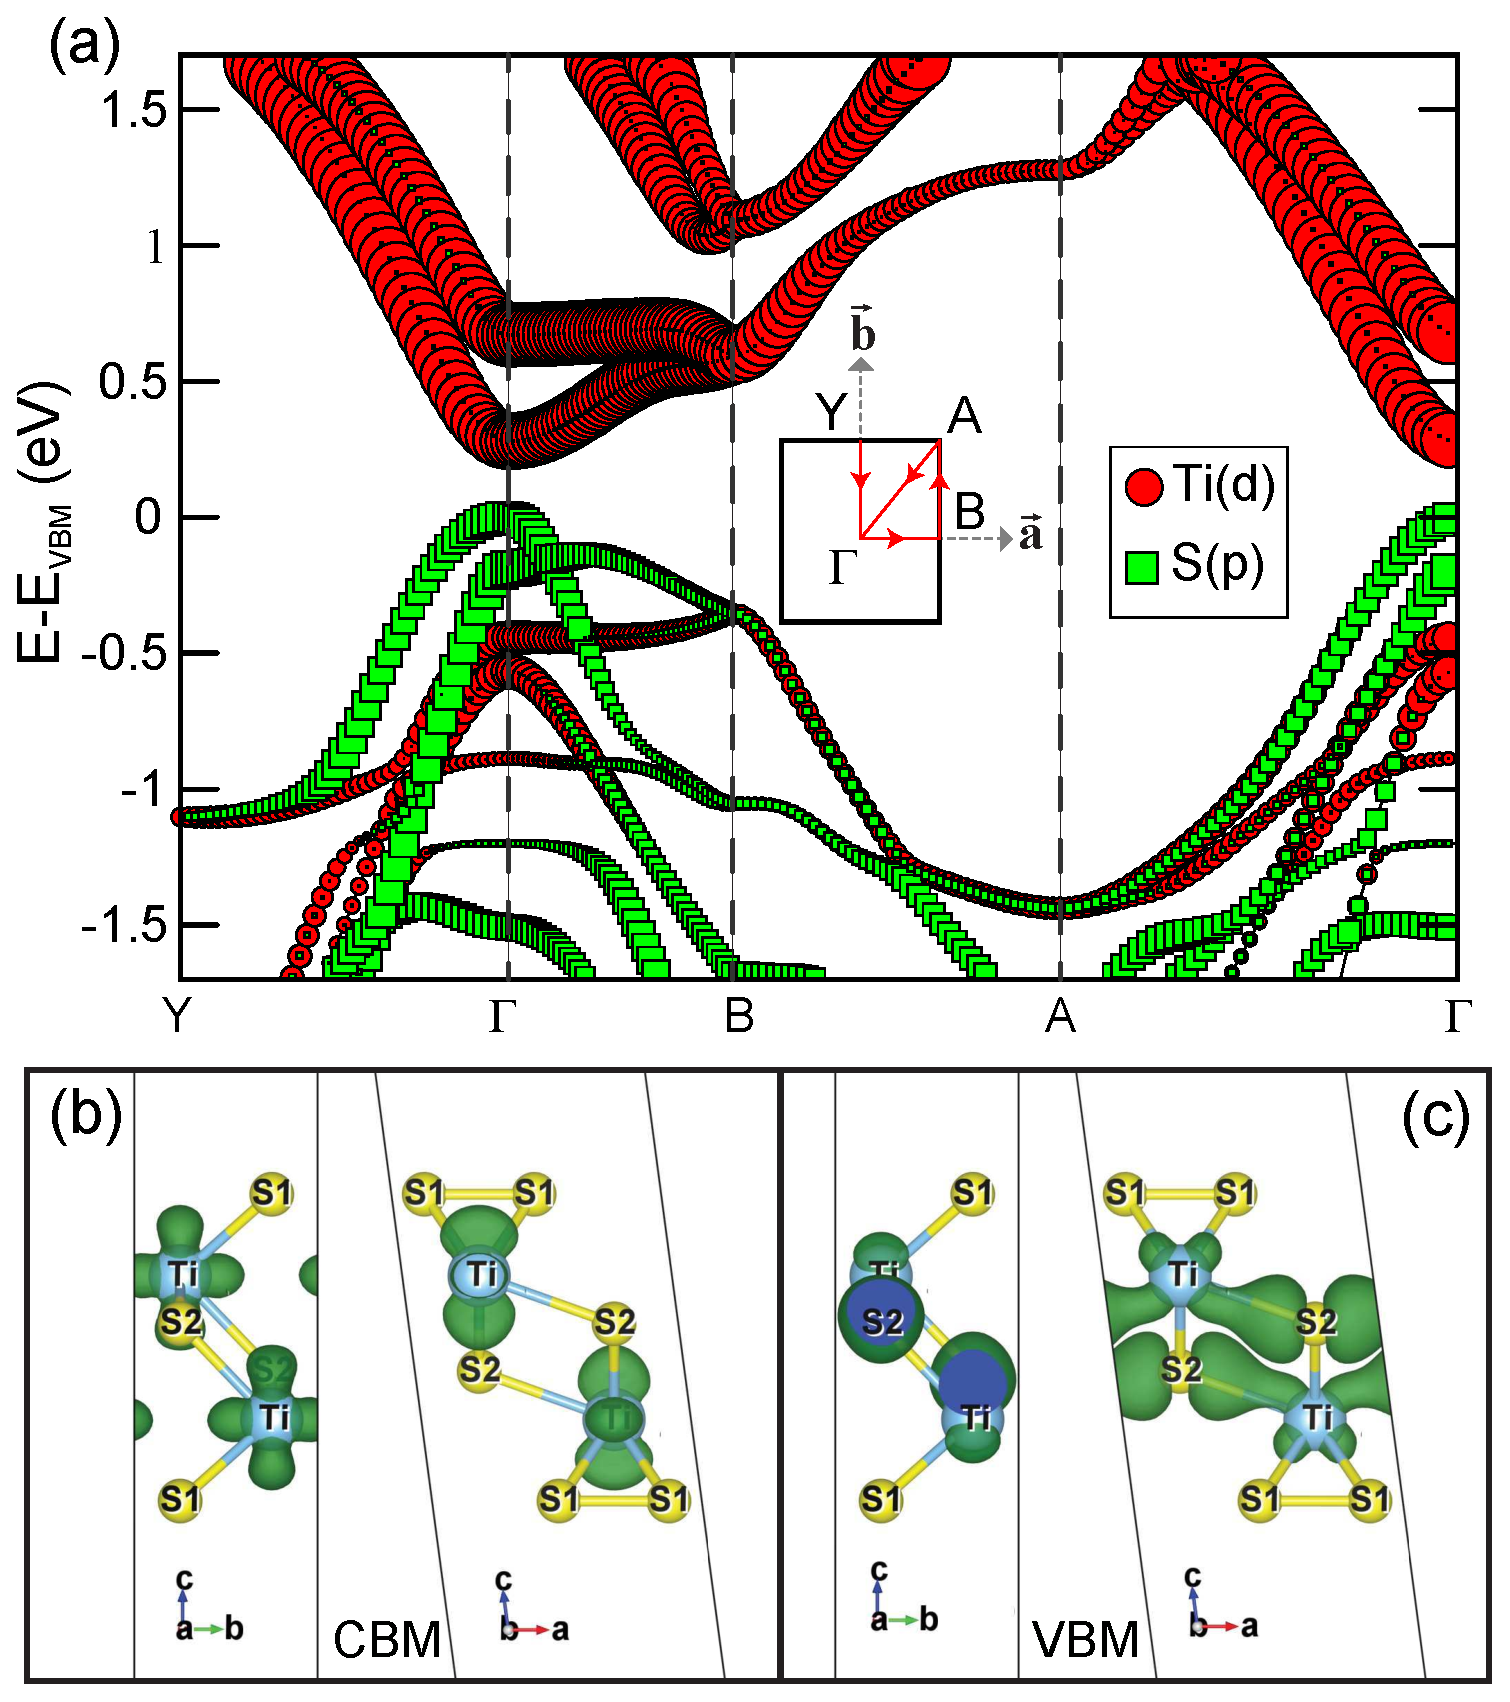
\includegraphics[width=0.8\linewidth]{Mob_projected_bands.eps}
\caption{(a) The site and orbital-projected band structure (calculated using PBE functional) of the unstrained TiS$_3$ monolayer.  Decomposed charge density of CMB (b) and  VBM (c) at the $\Gamma$ point are presented. \label{band} }
\end{figure}

As is shown in Fig.~\ref{band}, monolayer TiS$_3$ is a direct band gap semiconductor having a band gap of 0.29 eV (1.06 eV \cite{Dai2015}) calculated with PBE (HSE06) functional at the $\Gamma$-point.  The conduction band minimum (CBM) has the largest contribution from d$_{x^2-y^2}$ and d$_{z^2}$ orbitals of the Ti atoms, while the valence band maximum (VBM) is mostly dominated by the p$_x$ orbital of the S atoms and  the $d_{xz}$ orbitals of the Ti atoms. The $x$ and $y$ directions coincide with the \textit{a} and \textit{b} directions, respectively. The $z$ direction is taken perpendicular to the $xy$ plane. Later, we will discuss in detail how these states change their energies when they are exposed to the mechanical strain.

To gain deep insight about the binding nature in the TiS$_3$ monolayer, we calculate the Bader charges\cite{Bader1,Bader2,Bader3,Bader4}. According to the Bader analysis, each Ti atom donates 1.61 $e^-$ to eight S atoms surrounding it. Each of the surface S atoms, labelled as S1 in Fig.~\ref{band}, binds only with two Ti atoms and gain 0.34 $e^-$ net charge. Two of these S1 atoms form a covalent bond between them. While each of the S atom between two Ti layers, S2 in Fig.~\ref{band}, binds with four neighboring Ti atoms, and have 0.81 $e^-$ net charge accumulated on it.  The electronegativity differences between S (2.58) and Ti (1.54) is calculated as 1.04, which belongs to the polar covalent bond class \cite{David2015}.  This value is large as compared to that of MoS$_2$ where Molybdenum (2.16) and S (2.58), which is 0.41 and is considered as covalent bond type.

%\begin{table}[ht]
%\caption{The electron (hole) effective mass ($m^*$), the elastic modulus ($C$), the deformation potential constant ($E_d$), and the electron (hole) mobility ($\mu$) of phosphorene and monolayer TiS$_3$.}
%\centering
%\begin{tabular}{l|lcccccc}
%\hline\hline
%Material & Carrier type & Direction & $m^*$($m_e$) & $C$(N/m) & $E_d$(eV) &  $\mu$(10$^3$ cm$^2$V$^{-1}$s$^{-1}$)\\ \hline
%\multirow{}{}{Phosphorene} & electron & armchair & 0.20 & 24.30 & 0.65 &  1.93 \\
%& hole & zigzag & 6.89 & 103.14 & 0.11 & 25.36 \\ \hline
%
%\multirow{}{}{TiS$_3$ monolayer} & \multirow{}{}{electron} & \textit{a} & 1.52 & 82.68 & 0.53 & 1.82 \\
%&   & \textit{b} & 0.40 & 133.76 & 0.84 & 17.08 \\ 
%& \multirow{}{}{hole} & \textit{a} & 0.30 & 82.68 & 2.53 & 2.00 \\ 
%&   & \textit{b} & 0.99 & 133.76 & 4.10 & 0.11 \\ \hline\hline
%
%\end{tabular}
%\label{unstrain}
%%}
%\end{table}

Before  applying strain to our system, we summarize  the mobility and related parameters for the unstrained TiS$_3$ in Table \ref{unstrain}, which are in agreement with previous calculations \cite{Dai2015}. Similar data for phosphorene are presented for comparison. The results for phosphorene are recalculated with the same computational parameters as TiS$_3$. The mobility of the electron in TiS$_3$ monolayer has an impressive level, which is an order of magnitude larger than that in phosphorene. However, resulting from very small DPC, hole mobility in phosphorene is an order of magnitude larger than that in TiS$_3$.  Moreover, the anisotropy of the effective mass along different crystallographic directions is much more significant for phosphorene as compared to that in TiS$_3$. Phosphorene overall is softer than TiS$_3$ as far as the elastic modulus is concerned.

\subsubsection{Dynamical stability under  mechanical strain}

\begin{figure}[htb]
\centering
\includegraphics[width=0.7\linewidth]{Mob_stiffness.eps}
\caption{Calculated elastic modulus along the \textit{a} and \textit{b} directions under mechanical strain. \label{stiffness}}	
\end{figure}

Applying mechanical strain may have important effects on the stability of a structure. Therefore, it is crucial to know if  strain applied to the system does not induce any structural instability. To this purpose, we calculate the elastic modulus and phonon spectrum for the TiS$_3$ monolayer under various strain values in order to confirm its dynamical stability.  Figure~\ref{stiffness} shows the elastic modulus along the \textit{a}  and \textit{b}  directions as a function of applied strain. These values correspond to the elastic constants, i.e.  C$_{11}$ and C$_{22}$.  Here, C$_{11}$ (C$_{22}$) reflects the mechanical response of the TiS$_3$ monolayer to a strain applied along the \textit{a} (\textit{b}) direction.  The calculated value of C$_{11}$ (C$_{22}$) for the unstrained TiS$_3$ is 133.76 (82.68) N/m, in good agreement with previous calculations \cite{Dai2015,kang2015m}. Note that the calculated elastic constants are all positive and they fulfill the mechanical stability criteria, i.e. C$_{11}$ and C$_{22}$ $>$ 0. These results clearly imply that monolayer TiS$_3$ is less stiff than graphene and single layer h-BN, however, it is mechanically superior as compared to MoS$_2$ and phosphorene\cite{deniz2}. Furthermore, C$_{22}$ is always larger than C$_{11}$, meaning that the \textit{a} direction is stiffer than the \textit{b} direction. 

\begin{landscape}
\begin{figure}[htb]
\centering
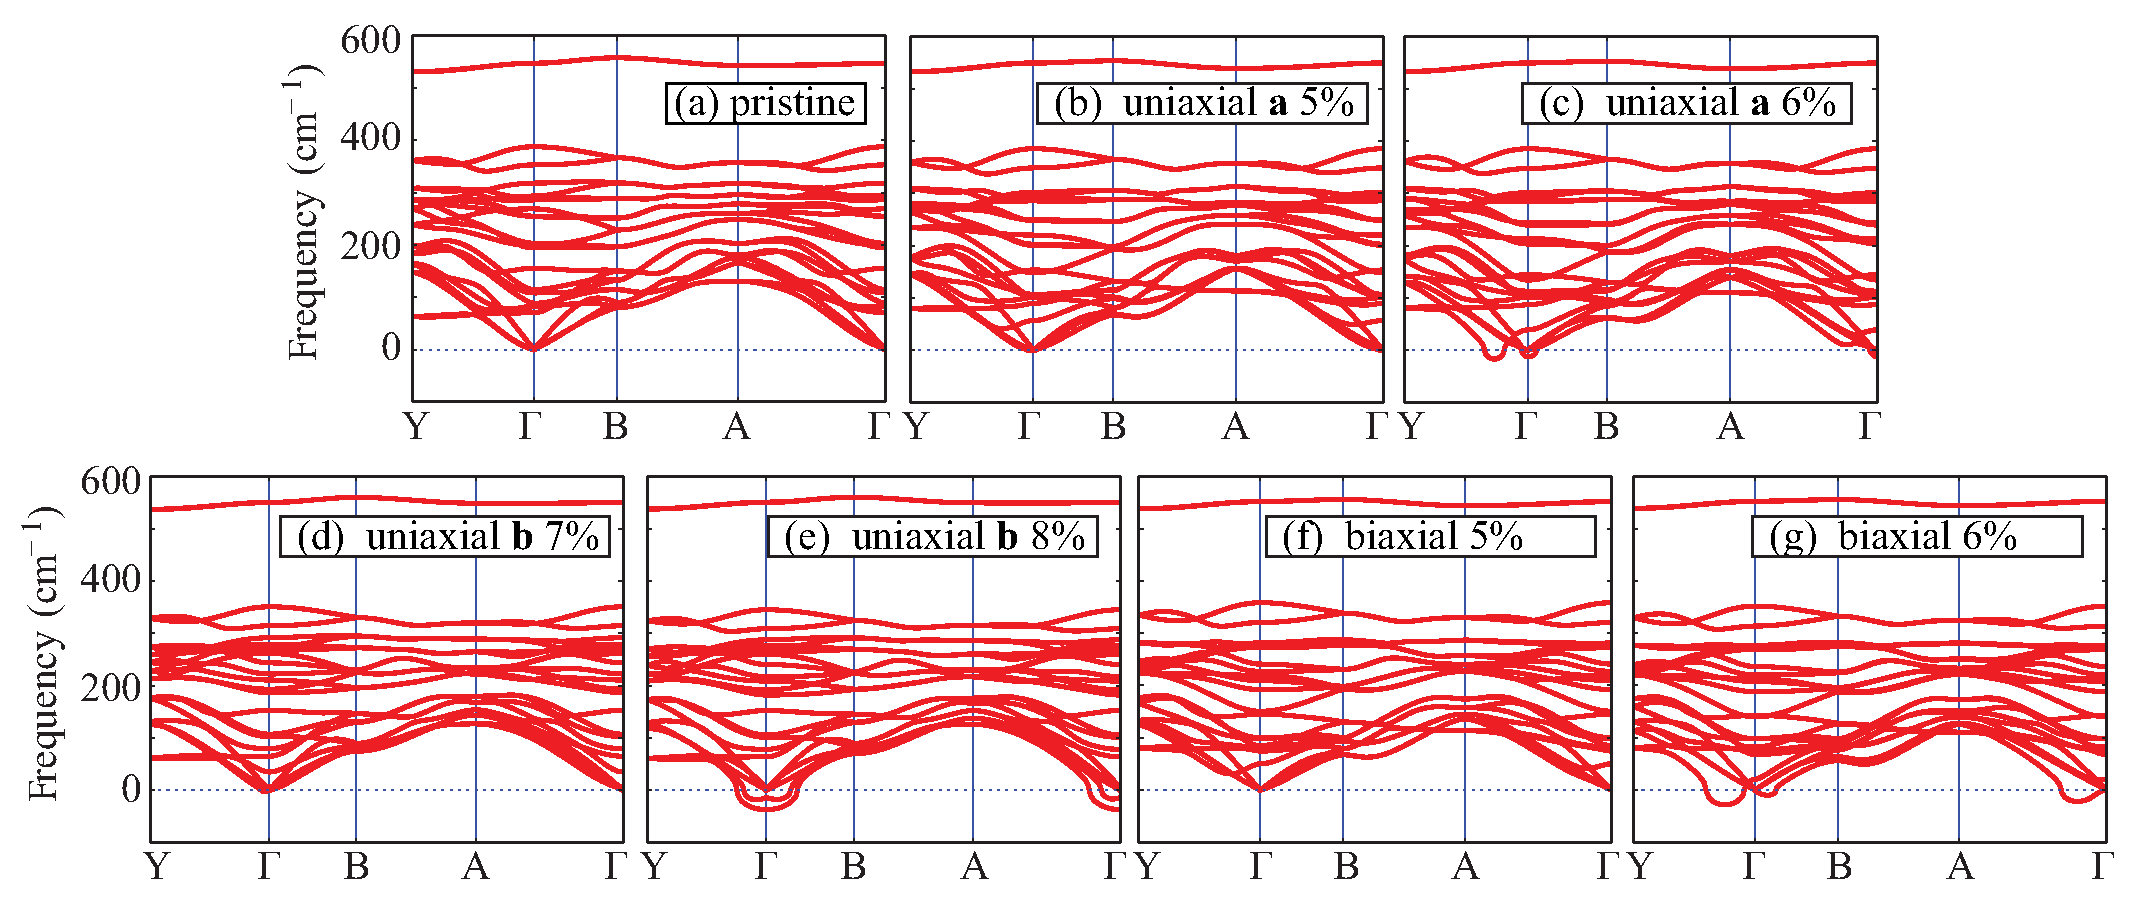
\includegraphics[width=\linewidth]{Mob_phn.eps}
\caption{Calculated phonon spectrum of (a) pristine monolayer TiS$_3$ and that under strain (b-g). }
\label{phn}
\end{figure}
\end{landscape}

In order to gain further insight into the stability of TiS$_3$ monolayer, we calculate the phonon dispersion under different types of strain. As shown in Fig.~\ref{phn},  uniaxial strain applied along the \textit{a} and \textit{b} direction induce dynamical instability in the system at strain values of 6\% and 8\%, respectively.  Note that the highest optical mode reaches up to ~550 cm$^{-1}$ and does not vary with strain. Consistence with our results of the elastic constants, the optical phonon modes are more sensitive to strain applied along the \textit{b} direction, see Fig.~\ref{phn}. Except for the topmost mode,  phonon branches move downward with strain applied along the \textit{b} direction.  We observe an average downward shift of 25 cm$^{-1}$ at 8\%, which should be easily detected by Raman spectroscopy.  The observed instability at large strain values is due to the presence of imaginary vibrational frequencies, suggesting a structural phase transition. The dynamical stable range of black phosphorus is 15\% which is much larger than that of TiS$_3$\cite{0953-8984-27-17-175006}.  Due to its puckered structure, the former is able to sustain large mechanical deformations.  The biaxial case is the combination of two uniaxial strains applied along the \textit{a} and \textit{b} directions, and the stable range is determined by the lowest strain value, i.e. 6\% applied along the \textit{a} direction. 

\subsubsection{Bond lengths and band gap under mechanical strain}
The foremost consequence of the mechanical strain is the change of the structure parameters in the unit cell. Strain is applied by manually changing the lattice constant along the desired direction. After that, the cell parameters are kept fixed whereas the internal atomic positions are allowed to fully relax. Therefore, the latter can be considered as the response of the material to the external strain, which would carry important information about the consequential effects. The variation of the bond length provides information about how the local environment of atoms in the unit cell changes with strain. Considering this, we plot the bond lengths with respect to the different types of strain in Fig.~\ref{bonds}. 

\begin{figure}[htb]
\centering
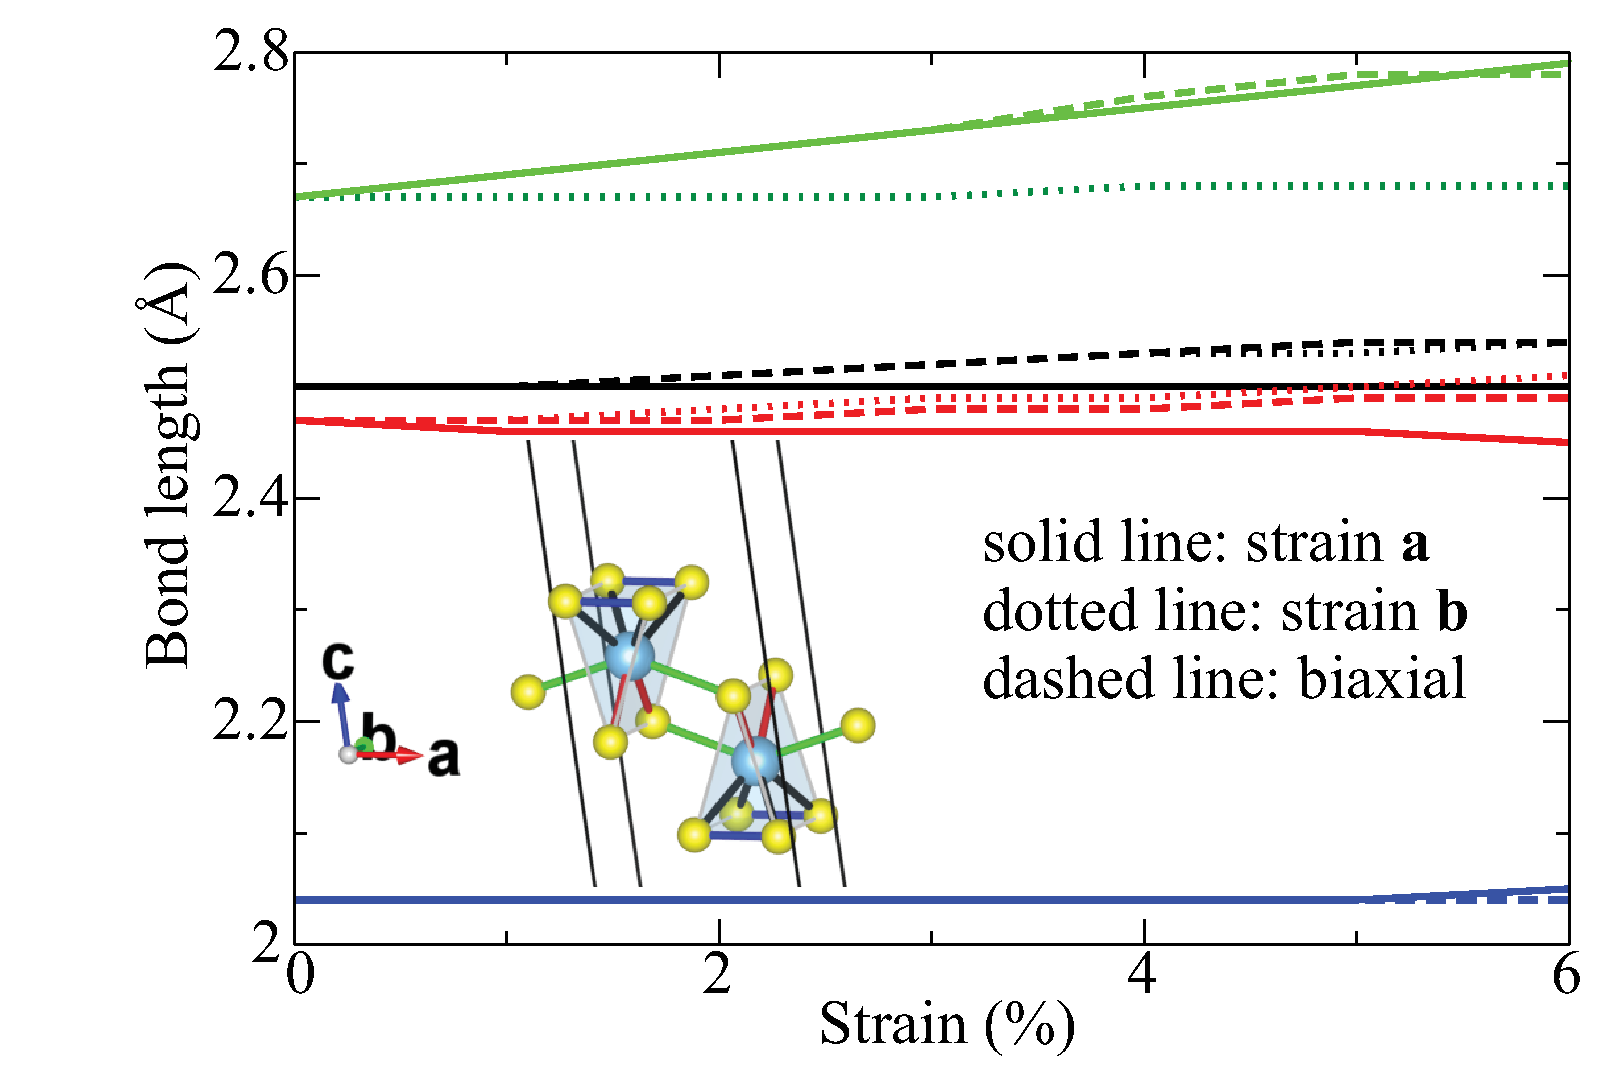
\includegraphics[width=0.9\linewidth]{Mob_bonds.eps}
\caption{Variation of bond lengths with strain. Color of the curves matches with the color of the bonds in the structure depicted in the inset.\label{bonds}}
\end{figure}


\begin{figure}[htb]
\centering
\includegraphics[width=0.7\linewidth]{Mob_bandedges.eps}
\caption{Variation of the band edges with respect to vacuum with strain. \label{bandedges}}
\end{figure}

In the following discussion, we correlate the variation of the CBM and VBM, as shown in Fig.~\ref{bandedges}, with the change of bond length by investigating their bonding character. Let us first focus on strain applied along the \textit{a} direction. The most significant change occurs for the Ti-S bond between two neighboring prisms. As the strain increases, the local environment inside the prism hardly changes, whereas the bond lengths of Ti-S bonds between prisms. On the other hand, it can be seen from the decomposed charge density of the VBM at the $\Gamma$ point for the unstrained TiS$_3$ (see Fig.~\ref{band}(c)) that the Ti-S distance between two prisms is controlled by the Ti-S bonding state at the VBM. Therefore, we would expect that the energy of this state increases (i.e. its binding energy decreases) with tensile strain, which can be seen in Fig.~\ref{bandedges}. For strain applied along the \textit{b} direction, one can note from Fig.~\ref{band}(c) that the VBM charge distribution along the \textit{b} direction has a node between two prisms. Given the fact that atoms sit close to each other, this is an  anti-bonding state. Therefore, we would expect that its energy decreases (i.e. its binding energy increases by depopulating the anti-bonding state) when strain along the \textit{b} direction increases. This is true when we see the trend of the VBM with the strain applied along the \textit{b} direction in Fig.~\ref{bandedges}. The CBM mostly gives a nonbonding state regardless of the direction, see Fig.~\ref{band}(b). This results in a much slower variation of the energy of  the CBM under tensile strain, yet only an overall small change is observed. 

Figure \ref{bandedges} also provides information about the variation of the band gap under strain, which agrees well with previous calculations \cite{Biele2015,Li2015}. While the band gap decreases under strain applied along the \textit{a} direction, it increases with strain applied  along the \textit{b} direction. The band gap increase in the latter case was experimentally confirmed \cite{Biele2015}.  By the help of  strain engineering, it is possible to tune the optical gap from far infrared to near infrared. The nature of the band gap remains direct within the considered tensile strain range where TiS$_3$ is dynamically stable. We find that  biaxial strain is a superposition of the above two situations as can be seen from Fig.~\ref{bandedges}. 

\subsubsection{Effective mass, deformation potential constant and mobility under  mechanical strain}

\begin{figure}[htb]
\centering
\includegraphics[width=0.7\linewidth]{Mob_emass.eps}
\caption{Variation of the effective mass of electron and hole along the \textit{a} and \textit{b} directions at the $\Gamma$-point with strain. \label{emass}}	
\end{figure} 

Using the computational setup described above, we estimate the acoustic-phonon-limited mobility of monolayer TiS$_3$ under  strain via Eq.~(\ref{equ}). According to this equation, at a particular temperature (e.g. 300 K),  three different physical parameters, namely elastic modulus $C$, carrier effective mass $m^*$ and DPC or $E_d$,  are subjected to a change under strain. Previously, we already discussed the variation of the elastic modulus with strain, which is shown in Fig.~\ref{stiffness}. Now we discuss how the effective mass and DPC change under strain. Figure \ref{emass} shows the effective mass of both hole and electron for different directions and strain values. All curves change monotonically. There is no abrupt change of the slope of the curves since there is no band crossing in the considered strain range, and one would expect a smooth variation for the band edges with strain. The electron mass along the \textit{a} direction increases regardless of the direction of applied strain, and the magnitude of this change is the largest among both carrier effective masses along the other directions. Because of this, the degree of anisotropy in the effective mass increases as TiS$_3$ is subjected to strain. As for the hole effective mass, the difference along the \textit{a} and \textit{b} directions increases for strain applied along the \textit{a} direction whereas this difference decreases for strain applied along the \textit{b} direction. Such anisotropy can be utilized to modify the electronic and thermoelectric properties of TiS$_3$.  

\begin{figure}[htb]
\centering
\includegraphics[width=0.7\linewidth]{Mob_dePotential.eps}
\caption{Variation of the (a) deformation potential constant ($E_d$) with strain. \label{dePotential}}
\end{figure}

Our calculations unveil that one of the most important  factors  that determines the mobility is the DPC.  In order to evaluate DPC, we need to apply a small dilation  along the direction where DPC is calculated. The ratio of the CBM (VBM) shift  to the amount of this dilation gives DPC for electron (hole), see Fig.~\ref{dePotential}. Mathematically, as shown in Eq.~(\ref{equ}), it is the square of a small number in the denominator. Thus the variation of DPC determines the whole ratio in Eq.~(\ref{equ}) thereby the mobility, unless other quantities change dramatically, which is not the case as we have discussed. For example, in the work of \citet{fei}, they reported the direction of the highest mobility change by 90$^{\circ}$, which was a result of the change in the smallest effective mass in a particular direction. In our case, we  observe no band crossing  and the variation of the  effective mass with strain is rather small for the highest mobility directions, see Fig.~\ref{emass}.   


%\textcolor{red}{Therefore, if the dilation direction is the same as strain direction, the DPC of electron (hole) variation should consist with the slope of the CBM (VBM) with respect to %strain.  As an example, we compare DPC for hole along the \textit{a} direction under strain applied along the same direction with the slope of VBM along the same direction in   
%\ref{bandedges}. The variations of the slope is clear enough for simple observation, and one can conclude that it decreases as the strain, thus we would expect the %corresponding DPC should also decrease as the same strain, which is the case in \ref{mo-de}(a).  As for the DPC variation of carriers on the direction that is differ from the %strain direction, e.g. DPC of the electron along the \textit{a} direction under the strain along the \textit{b} direction, there is no intuitive way as in the previous case to demonstrate %the reason for the variation. However, the accuracy of the calculation is confirmed from the consistent trends on the band edges and DPC in the previous case.}

\begin{figure}[htb]
\centering
\includegraphics[width=0.7\linewidth]{Mob_mobility.eps}
\caption{Variation of the mobility ($\mu$) with strain.\label{mobility}}
\end{figure}

Next, we explore the mobility variation under strain, see Fig.~\ref{mobility}. For uniaxial strain along the \textit{a} direction, the two most apparent changes are the moderate enhancement of the hole mobility along the \textit{b} direction, from 2.00$\times10^3$ to 7.08$\times10^3$ cm$^2$V$^{-1}$s$^{-1}$ and the drop of the electron mobility along the same direction, from 1.82$\times10^3$ to 0.25$\times10^3$ cm$^2$V$^{-1}$s$^{-1}$. Although the electron mobility along the \textit{a} direction for strainless TiS$_3$ is close to the hole mobility along the same direction, an order of magnitude difference can be realized by the help of tensile strain. Therefore,  uniaxial strain applied along the \textit{a} direction would be helpful to select carrier type based on their different transport properties.  For uniaxial strain along the \textit{b} direction, we find a dramatic enhancement of the electron mobility along the \textit{a} direction, from 1.71$\times10^4$  to 5.53 $\times10^5$ cm$^2$V$^{-1}$s$^{-1}$ at 300 K. This corresponds to a mobility enhancement from 5.13$\times10^4$ to 1.66$\times10^6$ cm$^2$V$^{-1}$s$^{-1}$ at 100 K. The subsequent drop at 7 \% can be ascribed to being close to the edge of the dynamical stable region. Furthermore, the electron mobility in the other direction (i.e. \textit{b}) has a moderate enhancement at strain value of 6 \% as well. The electron mobility along the \textit{b} direction has a considerable increase when tensile strain is applied along the \textit{b} direction. The hole mobility generally tends to decrease on both directions.  As stated before, the biaxial case is an effective combination of two uniaxial strains applied along the \textit{a} and \textit{b} directions. The electron mobility along the \textit{a} direction reaches up to  3.68 $\times10^5$ cm$^2$V$^{-1}$s$^{-1}$ at 5\% biaxial strain. 

Lastly, we discuss the effect of the optical phonon scattering on the mobility.  Using a Drude-like expression, $\mu$ can be expressed as  $\sim$ $q\langle\tau\rangle/m^*$, where $\langle\tau\rangle$ is the average scattering time, and in the Matthiessen's Rule, it is given as sum of all scattering process, i.e.  $1/\tau$=$1/\tau_{ph}$+ $1/\tau_{el}$+$1/\tau_{imp}$+ $\cdots$. Here, $\tau_{ph}$, $\tau_{el}$ and $\tau_{imp}$ are the scattering times related to electron-phonon, electron-electron and electron-impurity scattering, respectively.  In a rough estimate (i.e using Einstein's model), $\tau_{ph}$ for the longitudinal optical phonon scattering is inversely proportional  to the frequency of the optical modes. According to our calculations, the frequency of the phonon modes is subject to a redshift under strain. This means that the contribution of the optical phonon scattering reduces with increasing tensile strain.  As a result, we can claim that our trends are persistent against the contribution of the different scattering processes. 

\subsubsection{Summary}

In this work, we have demonstrated that, by the help of tensile strain, it is possible to enhance the carrier mobility of the TiS$_3$ monolayer more than an order of magnitude at 300 K and two orders of magnitude at 100 K. Phonon dispersion calculations revealed that TiS$_3$ becomes dynamically unstable for an uniaxial tensile strain larger than 6\% (8\%) applied along the \textit{a} (\textit{b}) direction. The degree of effective mass anisotropy can be controlled with uniaxial strain. The deterministic role of the deformation potential constant on the mobility in this material is confirmed. The variation of the CBM and VBM with strain was explained through the bonding character within the TiS$_3$ monolayer.  Here, we also showed that strain engineering appears as a quite exciting way to tune the electrical conductivity of TiS$_3$, which is potentially useful for device applications including flexible electronics.


\section{Heterostructures}

Another way to explore the property land of materials is to combine different composites to form heterostructurse\cite{Geim_Grigorieva_2013,Liu2016b,Pomerantseva2017}. They can be composites made by materials with complementary characters and perform better than each of the material individually, or materials those give new phenomenon and promising properties only when act together.  Given the obvious structure anisotropic in 2D materials, there are two types of heterostructures: vertical or lateral, see for example \autoref{fig:ver-lat-stru}. The vertical heterostructures composed of stacks of different 2D materials. They are held together via what holds graphite layers together: van der Waals force. Thus, this type of construction is referred as van der Waals heterostructures.  On the other hand, lateral heterostructure\cite{Jena2014,Chhowalla2015} is made by joining the edges of different 2D materials and the connection is mostly made through strong bonding, e.g. covalent or ionic. For this case, all the new properties results from the interface. In this section, I will present one for each type of the heterostructure and explore one properties. Comparisons will be made to illustrate the advantage of choosing these materials over the homo-structure. 

\begin{figure}[htb]
\centering
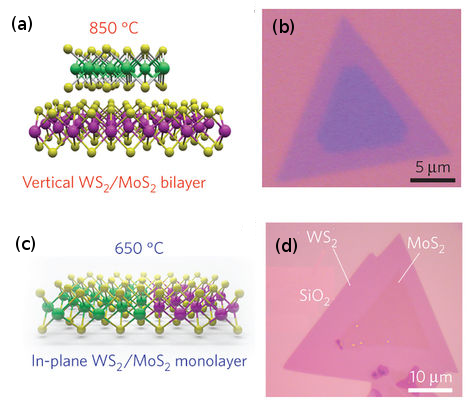
\includegraphics[width=0.9\textwidth]{ver-lat-stru.png}
\caption{ (a) and (d) vertical and (c) and (d) lateral WS$_2$/MoS$_2$ heterostructures. \label{fig:ver-lat-stru} Image adapted from: \cite{Gong_Lin2014}}
\end{figure}

\subsection[Electrical transport in 1T/2H/1T MoS2 lateral heterostructure]{Electrical transport in 1T/2H/1T MoS2 lateral heterostructure \footcite[This work is submitted as:][]{Aierken2017.transport}}

\subsubsection{Introduction}
Heterostructures are the essential components of a wide range of solid-state devices, such as transistors, solar cells, and sensors\cite{singh1993,agostini2011}. They are  fabricated by combining different type of materials, e.g. metal, semiconductor, and insulator. Therefore, the physical properties of the combined system are enhanced or become more controllable as compared to that of each material individually. These tailored properties are strongly related to the interface of two different materials where all interesting and new phenomenon occur. However, along with the emergence of nanostructured materials, dimensionality has become another major factor affecting the physical properties of materials and devices along with the interface. Thus, solid-state device fabrication with heterostructures based on low dimensional nanomaterials has attracted significant attention and a new research area in material design has been initiated where researchers are expecting unprecedented results, phenomenon and physics\cite{Gan2013,Wu2015c,DiBartolomeo2016}. Indeed, several advantages of two dimensional (2D) phase engineering over the three dimensional counterpart has already been demonstrated.\cite{Duerloo2015}

In low dimensional heterostructure device architectures, there are usually two types of interfaces connecting different materials: top contact (vertical) and edge contact (lateral)\cite{Allain2015}. In top contacts, an overlapping portion of two materials are glued together mainly via interlayer van der Waals (vdWs) interaction, while in edge contacts one dimensional edges of two materials are contacted with covalent bonds without overlapping. The van der Waals interaction in top contact introduces a potential gap between the two layers which electrons have to tunnel through, and resulting in higher resistance due to the reduced carrier transmission probability. Naturally, this resistance is much lower in edge contacts owing to the formation of covalent bonds that provides a path for carriers to travel across the interfaces\cite{Matsuda2010,Kang2014}. Recently, Eda \textit{et al.}  has discovered the coexistence of multi-phase MoS$_2$ that is a promising material for heterostructure device fabrication due to their natural metal-semiconductor-metal structure with clear edge contacts\cite{Eda2012}. Considering the distinct electronic nature of these phases, physical properties of these heterostructures\cite{Kappera2014,Fan2015} can be tuned by phase engineering and novel solid-state device architectures can be realized for several different future applications.

The same research group has synthesized two dimensional semiconducting heterostructure devices\cite{Huang2014,Zhang2015} by using metal contacts. As a result of their experimental analysis, they have particularly pointed out the vital importance of the geometry and electronic nature consistency between the metal contact and the heterostructure on the device performance\cite{Bai2013,Eda2012}. Considering this fact, Kappera \textit{et al.}\cite{Kappera2014} have locally induced 1T metallic phase of MoS$_2$ in the 1H semiconducting phase of it, and they measured that the edge resistance was lower than that of metal contacts by more than a factor of two. Subsequently, 1T$\mid$1H lateral heterostructure has been drawn peculiar attention as a promising contact structure having a higher carrier injection rate. Different arrangements of the interfaces between 1T and 1H phases was investigated through theoretical calculations\cite{Hu2015,Sivaraman2016} and the structure formed by the connection of armchair edges of 1T and 1H phases has been determined as an energetically more favorable configuration. However, in these calculations, the more stable metallic structure (1T$_d$), which arises with small distortion of 1T phase, was considered.

The present paper aims to investigate the electronic transport properties of MoS$_2$ multi-phase lateral junctions when the more stable metallic phase of MoS$_2$ ( i.e. 1T$_d$) acts as the contact, which is compared with the 1T phase. Further to this, the paper mainly focuses on the effect of doping on the electrical transport properties. In the results section, we first construct three junction models and calculate their transmission without external bias . Then we calculate the electronic properties for different level of doping.



\subsubsection{Computational details}
The presented first-principles calculations are based on density function theory as implemented in the Vienna $ab$ $initio$ Simulation Package (VASP) \cite{VASP1,VASP2,VASP3,VASP4}. A plane-wave basis set based on the projected augmented wave (PAW) method \cite{PAW1,PAW2} are used to describe the wave functions. The cutoff energy of the basis is set to 400 eV. Exchange-correlation interactions are treated with the generalized gradient approximation (GGA) within the Perdew-Burke-Ernzerhof (PBE) formulation \cite{GGA-PBE1,GGA-PBE2}. A 25$\times$25$\times$ 1 $k$-points mesh is used to sample the Brillouin-zone for monolayer structures of 1H, 1T and 1T$_d$ MoS$_2$ and a 9$\times$1$\times$1 $k$-points grid is used for the structures shown in Fig. \ref{structure-1t}. A vacuum space of 15 \AA~ is incorporated to avoid interaction between the periodic images. The energy convergence criterion for the self-consistent calculations is set to $10^{-5}$ eV, while the force convergence criterion for the ionic steps is set to $10^{-2}$ eV/\AA.

Electronic transport across the 1T$_d$/1T-MoS$_2\mid$1H-MoS$_2$ interfaces is calculated using the self-consistent non-equilibrium Green's functions (NEGF) technique as implemented in TranSIESTA\cite{transiesta} which is interfaced with the SIESTA code.\cite{siesta} Double-zeta (plus polarization) numerical orbital basis sets are used for all atoms. We employed norm-conserving pseudo-potentials\cite{tm}, the GGA/PBE functional, and an energy cutoff for the real-space mesh of 250 Ry.  In order to get accurate transmission spectra, the 2D Brillouin zone normal to the transport direction is sampled by meshes composed of  100 $k$-points in the periodic direction. While the SIESTA code uses a localized basis set and norm-conserving pseudopotentials, the calculated lattice parameters for different phases of MoS$_2$ agree well with those obtained from the VASP  code. 


\subsubsection{Results}
The use of metallic TMDCs as metal electrodes are expected to offer a breakthrough in the semiconductor industry as they have negligible heat dissipation and therefore are energy efficient. Among metallic TMDCs, metallic phases of MoS$_2$ (1T- and 1T$_d$-MoS$_2$) have attracted a growing interest due to its smooth interface with  the semiconductor phase of MoS$_2$ (1H-MoS$_2$). 
However, 1H phase is thermodynamically more stable than both 1T and 1T$_d$ phases. Therefore, the stabilization of 1T and 1T$_d$  over 1H phase becomes an essential requirement for the successful experimental realization of device configurable structures such as 1T/T$_d$-MoS$_{2}\mid$1H-MoS$_2$. On the other hand, 1T MoS$_2$ is the meta-stable and undergoes a Peierls transition to a low-energy state 1T$_d$ (or distorted 1T) and thus, metal contacts with the 1T$_d$ structure are more stable than the one with the 1T phase. However, the MoS$_2$ 1T$_d$ phase retransforms to the 1H phase at room temperature. 
As far as the relative stability is considered, choosing 1T$_d$ as metal contact further stabilized the junction.
Therefore, understanding the effect of different physical mechanisms on the stability of multiple phases (H, T, T$_d$) of this material is of vital importance to develop a proper control on phase transitions. To this end we mainly focus on the effect of doping (either charge or atom) on the stability, electronic and transport properties of 1T/T$_d$-MoS$_2\mid$1H-MoS$_2$ interfaces.  For the 1T and 1H hexagonal unit cells, the optimized in-plane lattice constant is obtained as 3.18 {\AA} .  On the other hand, the optimized lattice constants are $a$=3.18 {\AA}  and  $b$=5.72 {\AA} for  the tetragonal 1T$_d$ unit cell. 
These values are in good agreement with previous calculations\cite{C5NR07715J}. It was previously discovered the coexistence of 1T$_d$ phase with other two phases indicating their experimental stabilities, yet it is also possible to  relax the 1T$_d$ phase to to 1T phase using external source, such as electron beam irradiation\cite{Eda2012}. 
In experiment, 1T and 1T$_d$ are indistinguishable, because the S atoms are the same in two cases, only the Mo form cluster which STM image is limited to differentiate.


In this work, we systematically investigate the electronic and transport properties of three different device architectures, called as $\alpha$, $\beta$, and $\gamma$, denoted in Fig. \ref{structure-1t}.  In all device models, the semiconducting 1H-MoS$_2$ phase is sandwiched between two 1T$_d$ metal electrodes to create Schottky contacts at the interfaces. In the $\alpha$ structure, the metallic part consists of both 1T and 1T$_d$-MoS$_2$ phases. The size of metallic and semiconducting parts are larger than 20 {\AA} along the transport direction. The interface between the 1T$_d$-MoS2 and 1H-MoS$_2$ phases have either an armchair termination as in the case of   the $\alpha$ and $\beta$ structures, or a zigzag termination as in the case of the $\gamma$ structure in order to investigate the influence of the contact type on the calculated properties. We predict that the $\gamma$ structure significantly deviates from planar geometry after structural relaxation, see Fig. \ref{structure-1t}. To check whether such distortion is due to a calculation artifact, we started from a complete planar geometry and allowed both atomic coordinates and cell parameters relax to their equilibrium values (or lowest energy configuration). We observed that planar structure is not stable and structural relaxation brought back the original distorted structure. Indeed, such buckling or deviation from planar structure mainly restricts to the left interface, in line with a recent work that proposed a new crystal structure model for MoS$_2$\cite{C5NR07715J}.  Observed buckling helps to reduce repulsive interaction between S atoms at the left interface, thereby enhancing the stability of this interface.  

\begin{figure}[htb]
\centering
\includegraphics[width=0.8\linewidth]{structure.eps}%
\caption{\label{structure-1t}  Device models where 1H phase of MoS$_2$ is sandwiched between metallic MoS$_2$ electrodes. In (a) the $\alpha$-device, (b) the $\beta$-device, and (c)
the $\gamma$-device. For the $\alpha$ and $\beta$ devices, 
the interfaces between metallic and semiconducting MoS$_2$ have an armchair termination while a zigzag termination in the $\gamma$-device. }
\end{figure}


\begin{figure}[htb]
\centering
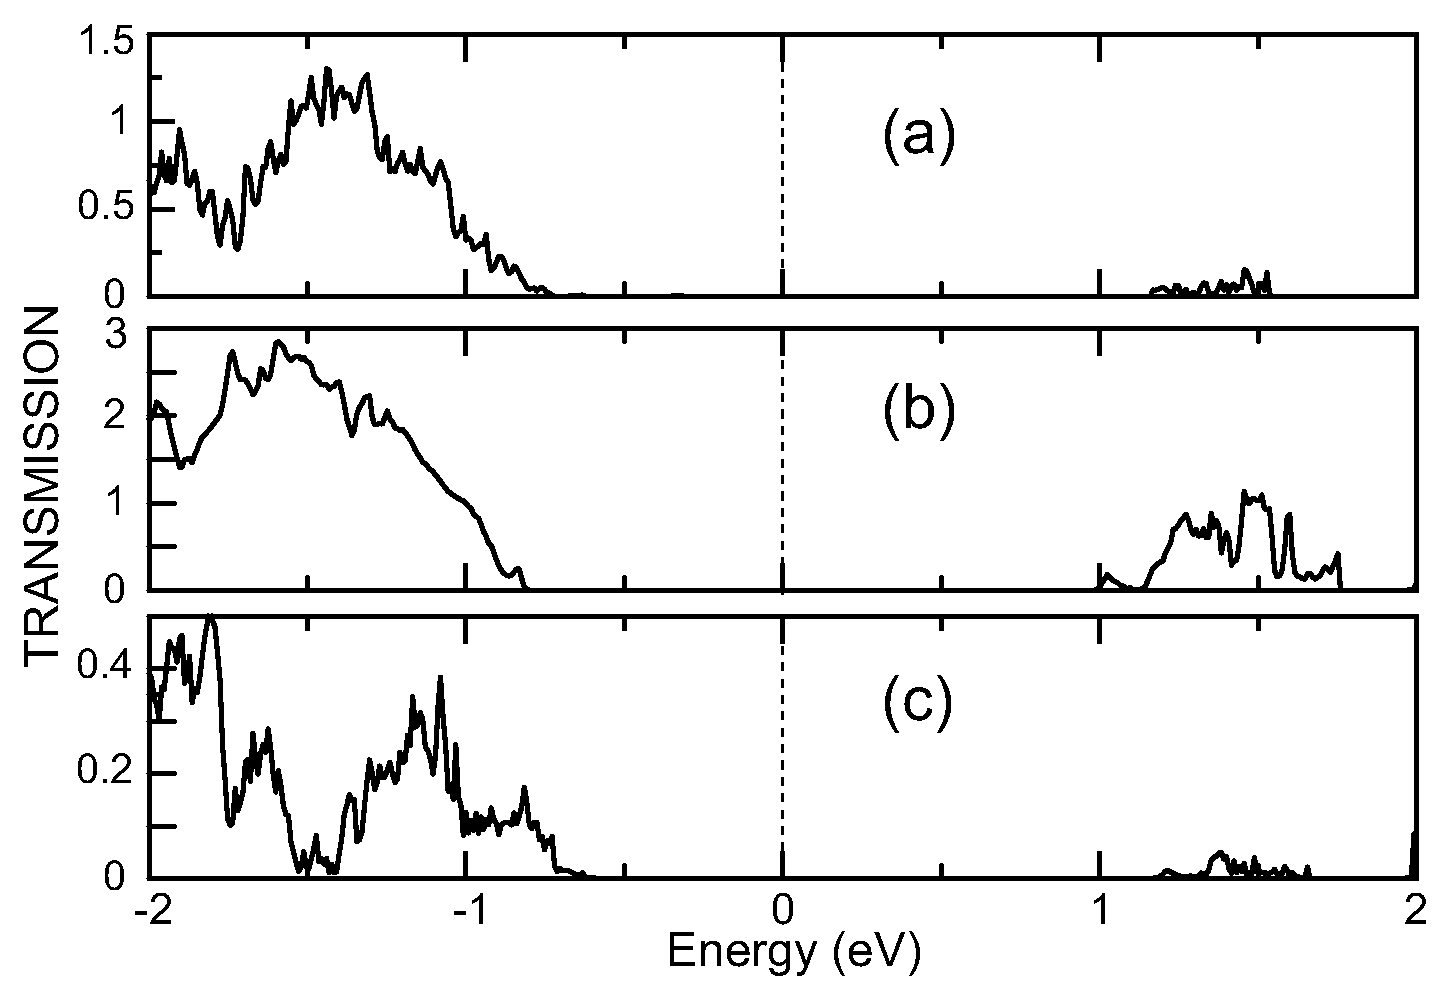
\includegraphics[width=0.8\linewidth]{TRANSMISSION-ALL-STRUCTURES.eps}%
\caption{\label{transport} The zero bias transmission spectra for (a) the $\alpha$-device, (b) the $\beta$ device, and (c) the $\gamma$-device. }
\end{figure}

The transmission spectra for all three  device models at zero bias are depicted in Fig.~\ref{transport}. In these plots, the Schottky barrier for holes (electrons) is defined as the difference between Fermi level and valence band maximum  (conduction band minimum) of the semiconductor 11HH phase of MoS$_2$. The first clear observation is that there is a large barrier height at the pristine interfaces and there is no transmission within an energy range of 1.8 eV around the Fermi level, corresponding to the band gap of 1H-MoS$_2$. The Schottky barrier heights for the $\alpha$, $\beta$ and $\gamma$ structures are predicted as 0.72,  0.80, and 0.63 eV for holes and 1.16, 0.99 and 1.19 eV for electrons, respectively. The estimated size of the scattering region along the transport direction is larger than 23 {\AA}, which is much smaller than the mean free path of electron in MoS$_2$\cite{mos2-trans} and therefore, the transport properties of these systems can be estimated with ballistic transport calculations. The $\beta$ structure has the largest transmission over the calculated energy range. The Mo atoms form a zigzag chain perpendicular to the interface (or along the transport direction) in the $\beta$ and also $\gamma$ structures which enhances the electrical transport in these systems. However, the non-symmetric Mo zigzag chain lying parallel  to the transport direction leads to scattering of electrons at the interface and gives rise to low transmission as compared to the $\alpha$ and $\beta$ structures. Similar anisotropic electron transport has also been  observed for ReS$_2$ where resistance is the lowest along the Re cluster direction\cite{doi:10.1021/acsnano.5b04851}. Comparing  the $\alpha$ and $\beta$ devices,  the coexistence of 1T and 1T$_d$ regions in the former device contributes to lowering of the transmission due to additional scattering at the 1T/1T$_d$ interface as compared to the latter device where we only have 1T$_d$ phase in the electrode region.

\begin{figure}[htb]
\centering
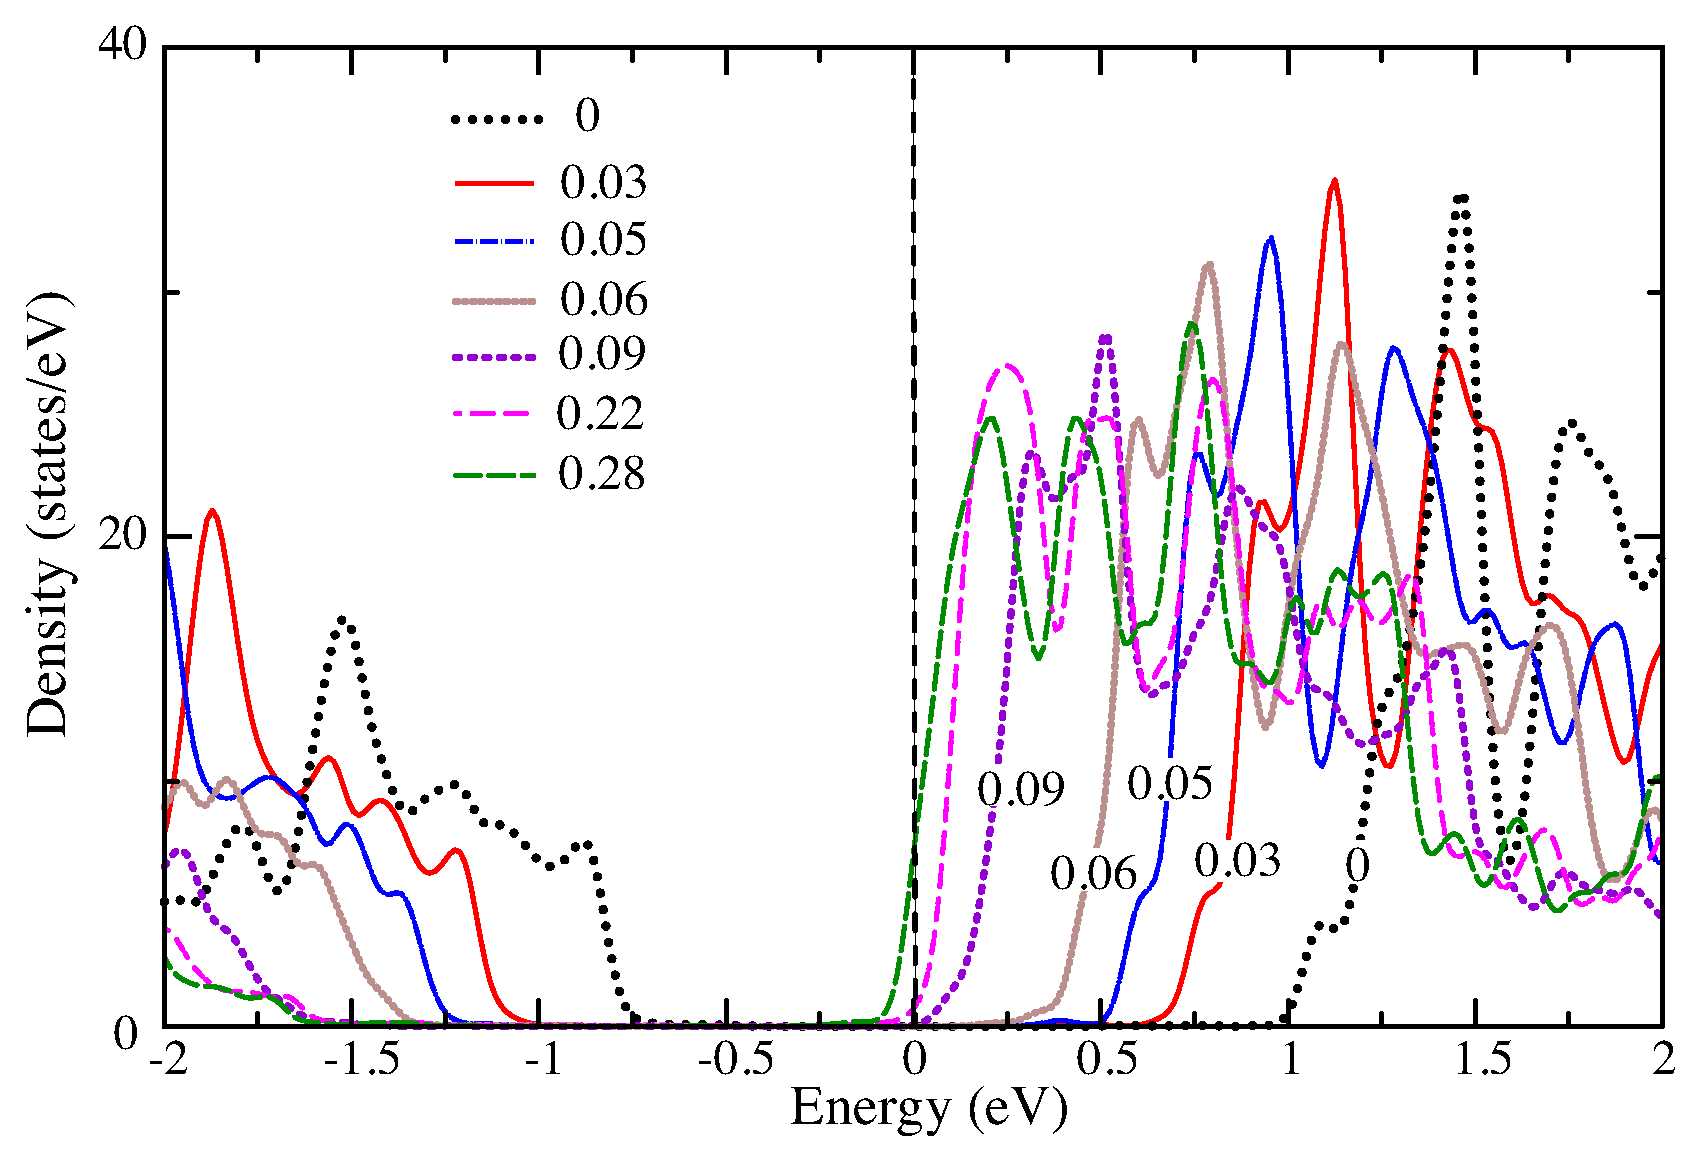
\includegraphics[width=0.8\linewidth]{dos-charge.eps}
\caption{Projected density of states of the valence and conduction band of 1H-MoS$_2$ as a function of electron concentration for the $\beta$-device. Here, we only show the PDOS of the central part of 1H-MoS$_2$ where the effect of the interface is minimal.  The Fermi level marks the zero energy. Electron concentrations (per formula unit of 1T$_d$ phase) are given. }
\end{figure}

\begin{figure}[htb]
\centering
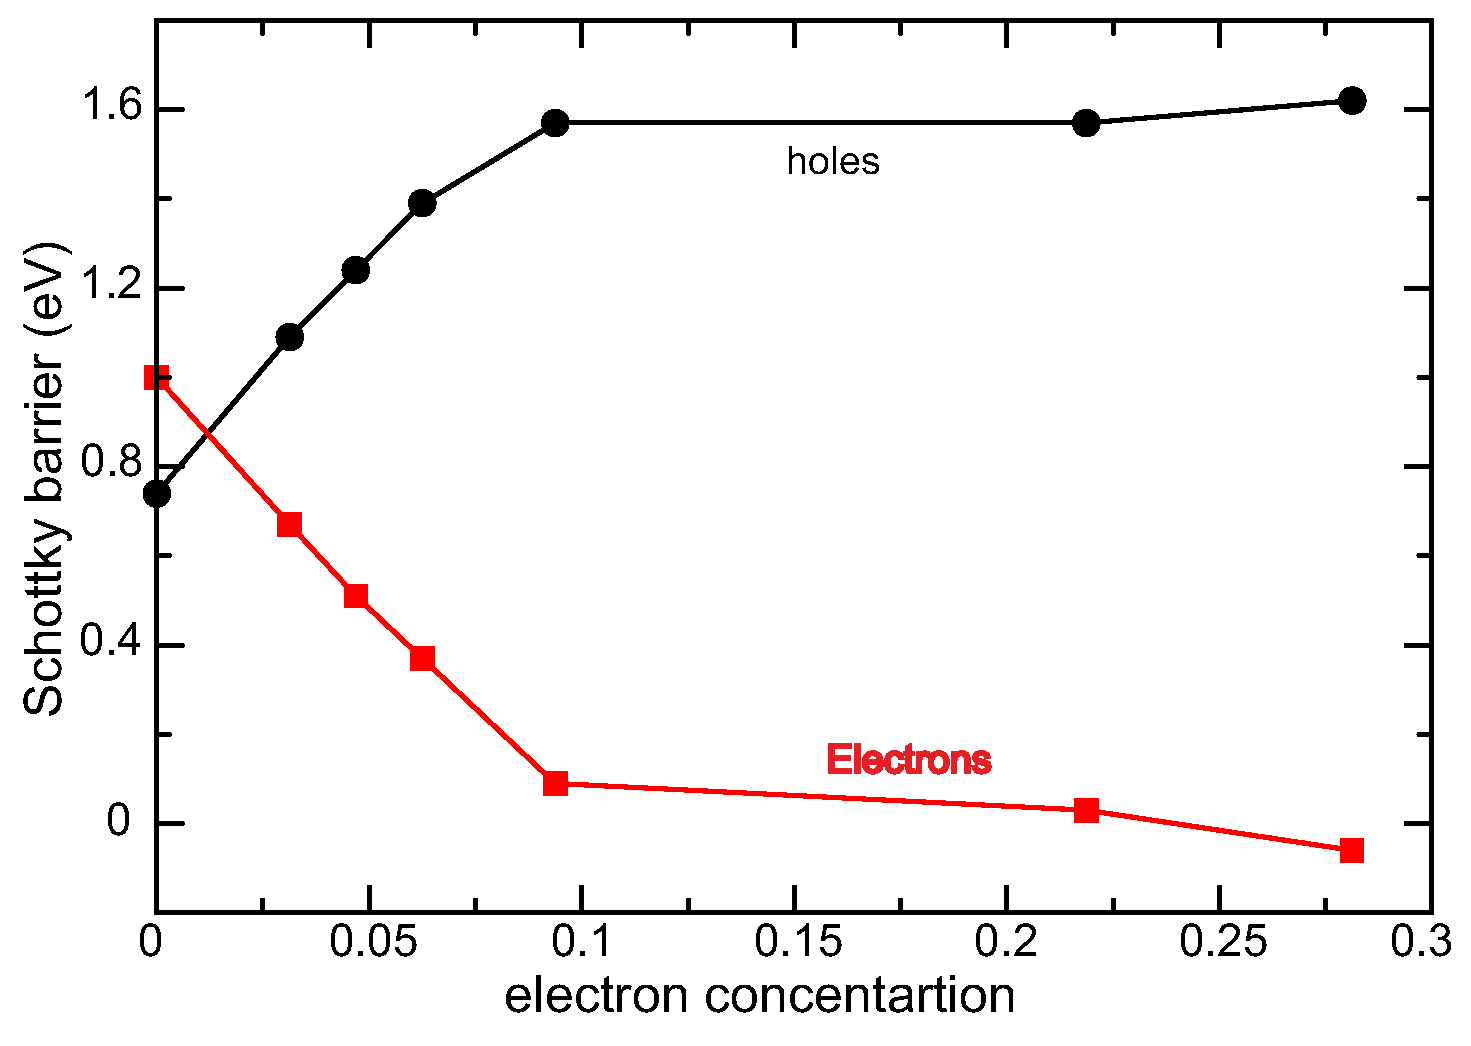
\includegraphics[width=0.8\linewidth]{Schottky-Charge.eps}
\caption{\label{sch-chg}Variation of Schottky barrier for the $\beta$-device as a function of electron concentration (per formula unit of 1T$_d$ part) for both electrons (red) and holes (black).}
\end{figure}

We next turn to the calculations of the electronic properties as a function of doping.
The central part of 1H-MoS$_2$ as the least affected from interface formation is considered to predict the band gap and the position of the band edges with respect to the Fermi level. The calculated band gap value, 1.75 eV,  clearly indicates that the size of the 1H part is large enough to achieve the monolayer limit and eliminates the electrode-electrode interaction. 
In fact, the band gap of the pristine 1H-MoS$_2$ monolayer calculated with the same functional is around 1.7 eV. 
In line with the transport calculations, the Fermi level appears within the band gap of the central region of 1H-MoS$_2$. The calculated Schottky barriers are 0.75 eV for holes and 0.99 eV for electrons in the $\beta$ structure. In the following discussion, we mainly focus on the $\beta$ structure due to its better transport properties as compared to the  $\alpha$ and  $\gamma$ devices. Other device models also exhibit similar properties. Our results contradicts experimental findings in the sense that, in experiments, it was shown that 1T (or 1T$_d$)$\mid$1H-MoS$_2$ interfaces exhibit a superior performance over the 3D metal-MoS$_2$ interfaces. However, we predict large Schottky barriers which give rise to a large contact resistance. In order to shed light on this contradiction, we calculate the electronic properties of the $\beta$ structure as a function of electron doping.   First of all, the electron doping stabilizes the 1T$_d$ phase over the 1H-MoS$_2$ and prevents the structural phase transition to the semiconducting 1H-MoS$_2$ phase\cite{doi:10.1021/jp4076355}. Also, the electron doping decreases the Schottky barrier height for electrons at the interface, leading to the formation of $n$-type Schottky barrier. This is attributed to the increase of the density of electrons in the $d$-orbital of the metallic 1T$_d$ MoS$_2$ phase.  Figure \ref{sch-chg} shows the variation of the Schottky barrier as a function of the electron concentration. We find that the Schottky barrier already diminishes for electron concentration larger than 0.1 electron (per 1T$_d$ MoS$_2$ formula unit). The Fermi level rises about 1 eV when only 0.28 electron is placed on the 1T$_d$ part. The direct electron doping can be achieved by using electron beams in experiments or Li/Na adsorption on the metallic phase\cite{doi:10.1021/acs.nanolett.6b01186,doi:10.1021/jp4076355} . Here, the considered alkali atoms donate their electron to the 1T$_d$ phase and enhance the stability and electronic properties of the metallic part\cite{doi:10.1021/jp4076355}. In addition, absorption of hydrogen atom on the 1T part of MoS$_2$ has been also shown to reduce the barrier at the interface of 1T-MoS$_2\mid$1H-MoS$_2$\cite{doi:10.1021/acs.nanolett.6b03999,doi:10.1021/acs.chemmater.5b00986}. 

Another possible strategy to enhance stability of metallic phases and electrical conduction at the metal-semiconductor MoS$_2$ interface is to dope metallic phase with transition metal atoms. Most of the well known TMDCs are either in the 1H or 1T phase when in their ground state. However, the single layer ReS$_2$ has neither H nor T as ground state, it stabilizes in 1T$_d$ structure\cite{tongay-res2,res2-cakir}. Therefore, alloying MoS$_2$ with Re may stabilize the 1T$_d$ structure of MoS$_{2}$ and leads to $n$-type doping of the crystal as similarly proposed by Raffone \textit{et al.} for Sn doped 1T phase\cite{Raffone}.  Meanwhile, we have previously shown that doping of ReS$_2$ with Mo results in a $p$-type doping of ReS$_2$ monolayer\cite{res2-cakir}. Therefore, we investigate the effect of substitutional doping of Re at Mo sites of 1T$_d$-MoS$_2$ on the transport properties. Here, we also consider the group V element Ta since the pristine TaS$_2$ monolayer crystallizes in the 1T phase and results in  a $p$-type doped 1T$_d$ MoS$_{2}$ structure. Indeed, in a recent work, it was shown that distorted phase of MoS$_2$ becomes energetically stable over 1H phase when Re concentration exceeds 50\%\cite{doi:10.1021/acs.jpcc.5b10739}. In this work, we did not consider such large dopant concentrations because of two reasons. First of all, lattice mismatch between 1H-MoS$_2$ and doped 1T-MoS$_2$ phases can be kept minimal for small dopant concentrations. At large concentrations, the relaxation of cell parameters leads to artificial enlargement of lattice parameters of  1H-MoS$_2$.  Secondly, Re doped 1T$_d$-MoS$_2$ becomes a semiconductor. To show the effect of doping, we only considered concentrations smaller than 20\%.  In this work, we assumed that doping of 1T-MoS$_2$ with Re or Ta may avoid the structural transition to 1H phase due to, for instance, temperature effect.  Figure \ref{re-ta-bare-dos} shows the PDOS for the central part of 1H-MoS$_2$ for Re and Ta doped $\beta$ structure. In the case of Re doping, the Fermi level approaches the conduction band of 1H-MoS$_2$, accompanying a significant decrease in $n$-type Schottky barrier height. On the other hand Ta doping reduces the $p$-type Schottky barrier height as expected. For a concentration of 14\% (per electrode), the $n$-type Schottky barrier becomes 0.85 eV for Re and $p$-type Schottky barrier becomes 0.58 eV for Ta.

\begin{figure}[htb]
\centering
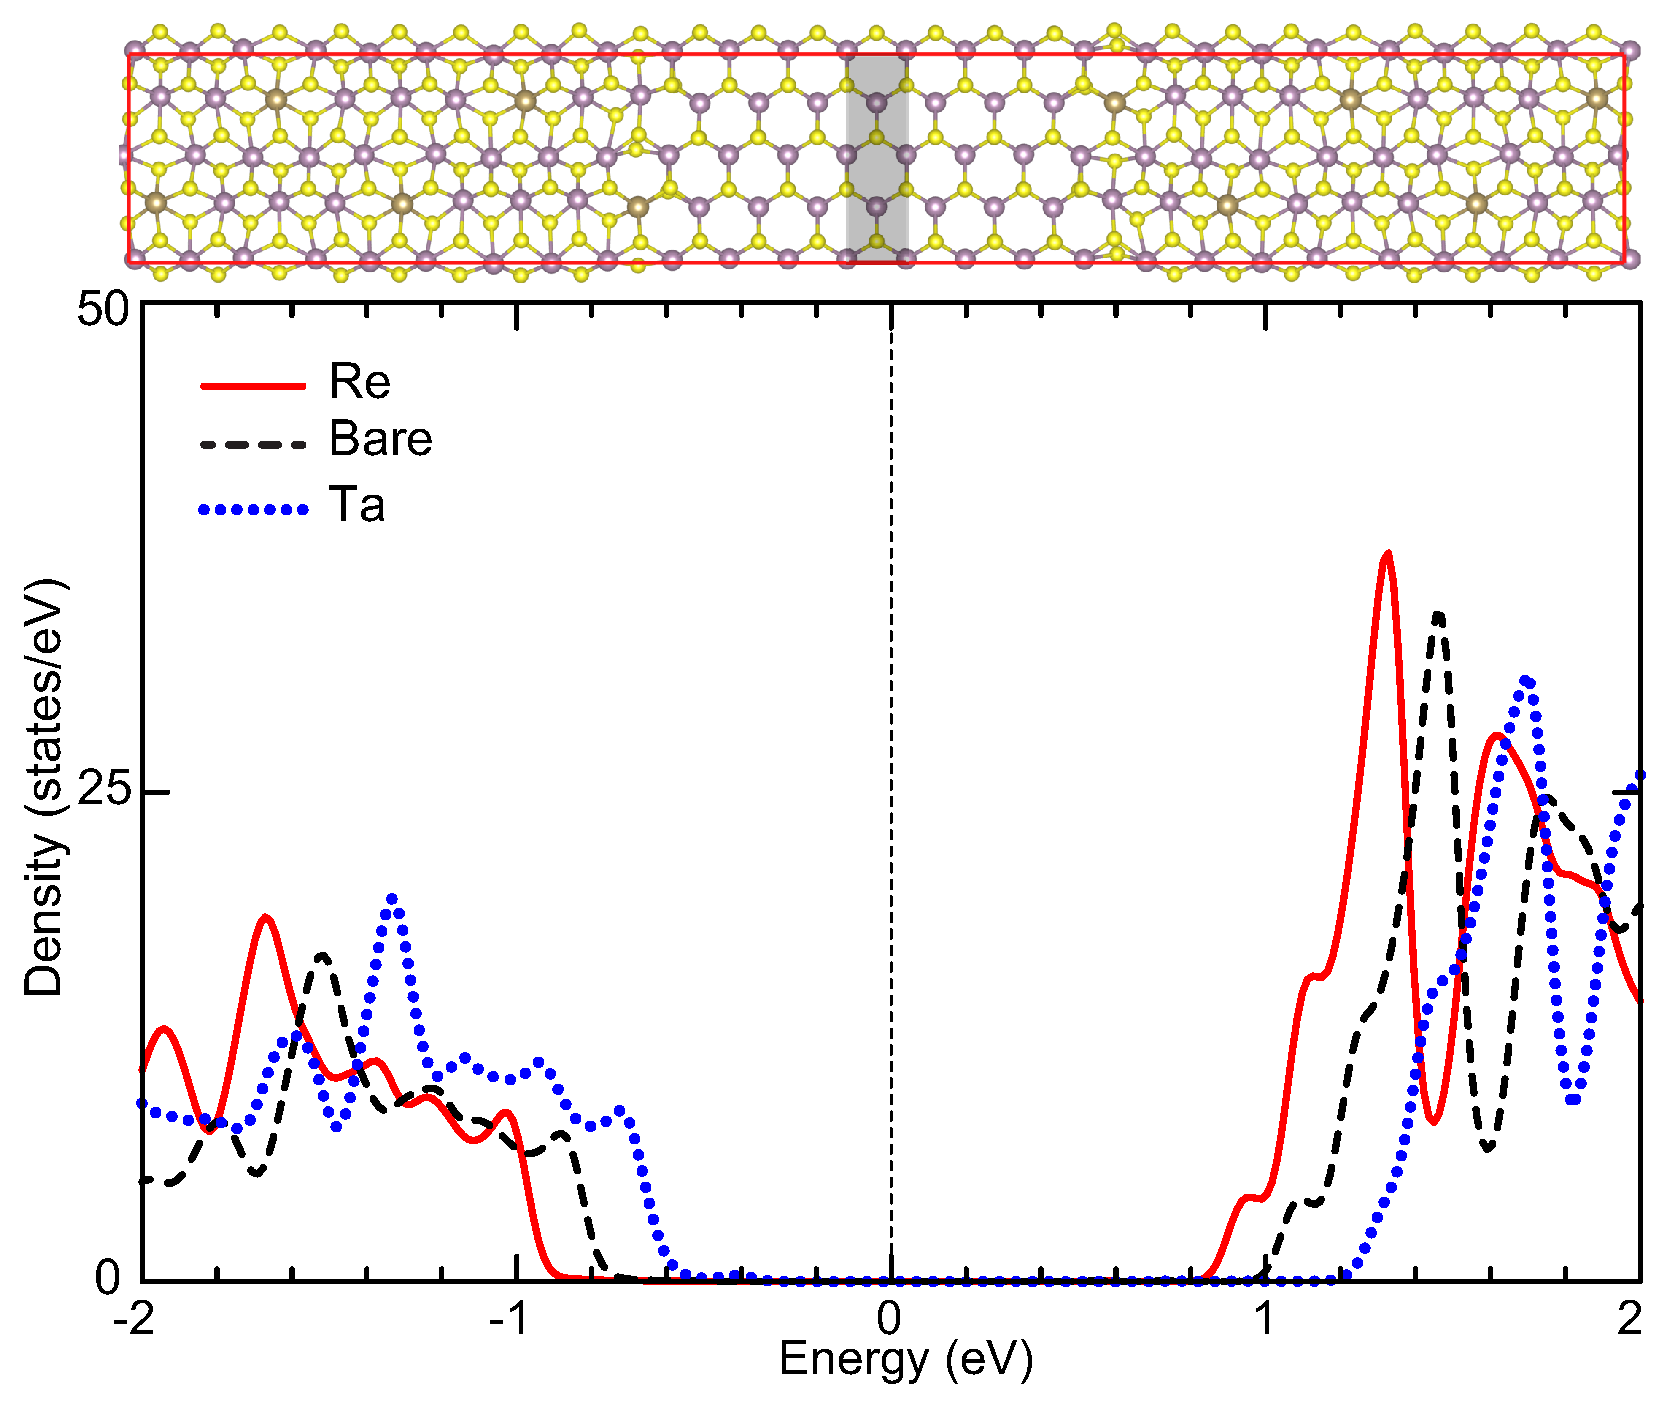
\includegraphics[width=0.8\linewidth]{Re1-Ta1-Bare.eps}
\caption{\label{re-ta-bare-dos}Projected density of states of the valence and conduction band of the central part of 1H-MoS$_2$ for Re and Ta doped devices. In the top figure, gray region highlights  the central part of 1H phase for which PDOS is calculated.  For comparison, PDOS of bare device is also shown.}
\end{figure}

\begin{figure}[htb]
\centering
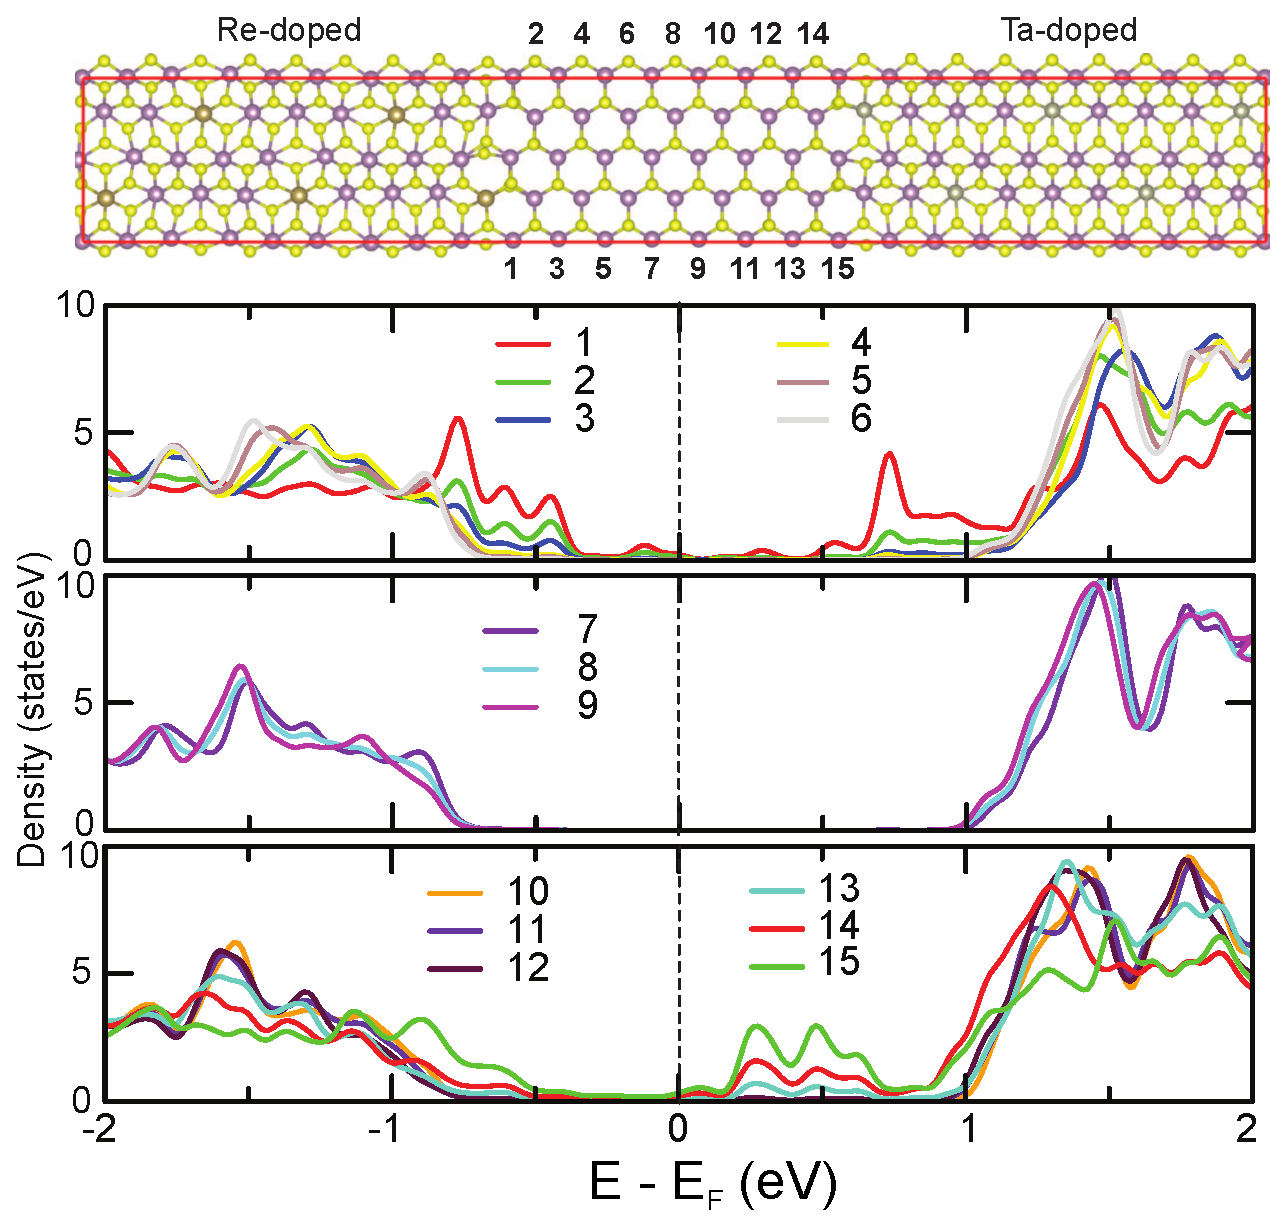
\includegraphics[width=0.8\linewidth]{pn-doped.eps}
\caption{\label{pn}Projected density of states of 1H-MoS$_2$ at the different position on 1H-MoS$_2$. 
The Fermi level marks the zero energy.}
\end{figure}

Since Re and Ta doping give rise to different electronic properties, we can design metal-semiconductor
junctions with different type of Schottky barrier heights (i.e. $n$- and -$p$ type) in the same device geometry. This allows us to design 
optical and photovoltaic applications. While a Re doped junction effectively blocks holes, Ta doped junction hampers the easy passage of electrons across the junction. In this device geometry, we can separate  photo-generated charge carriers for instance. Figure \ref{pn} shows the device model and projected density of states as a function of position in 1H-MoS$_2$. While the left electrode is doped with Re, the right electrode is alloyed with Ta.  The central part of 1H-MoS$_2$ clearly has a PDOS similar to free standing 1H-MoS$_2$ monolayer with a band gap of 1.75 eV.  However, we have different electronic properties in the right and left side of the central region.
Due to Re (Ta) doping, the left (right) part has a $n$ ($p$)-type Schottky barrier.  
The presence of 1T$_d$-1H MoS$_2$ interfaces develops mid-gap states that mainly come from the atoms in the
boundary region. The electronic properties gradually change from the metallic to the semiconductor when moving away from the interfaces.  For the atoms far away from the interface region (i.e. central region of 1H-MoS$_2$), we observe a clear band gap which is close to that of pristine 1H-MoS$_2$. While the mid-gap states appear below the Fermi level at the left interface (Re-doped side), they are unoccupied and reside above the Fermi level at the right interface (Ta-doped side).  About 3.2 {\AA} from the interface, the mid-gap states start to disappear.  

Figure \ref{potential} shows the electrostatic potential along the heterojunction. We consider both pristine and doped $\beta$-devices. 
For undoped heterojunction, the average potential is symmetric at the left and right interfaces.
However, doped heterojunction has a  different electrostatic potential, especially, within 1H-MoS$_2$. 
Due to its valence configuration, Re (Ta) acts as a donor (an acceptor). 
This is reflected in the average effective potential shown in Fig.~\ref{potential}(b).
The average electrostatic potential (EP) does not have a sharp variation at the 1T$_d$-1H interface, extending along the 2-3 atomic rows.  
This is due to fact that we form interfaces between two different crystal structures of MoS$_2$ (i.e 1T$_d$ and 1H). EP converges to  the same value at the left and right electrodes. 
If one considers a photovoltaic device using the  $\beta$ structure co-doped with Re and Ta, 
an electron-hole pair is generated after absorbing a photon in the 1H part. 
Re-doped interface has a higher potential as compared to Ta-doped interface, producing a driving force for dissociation of the electron-hole pair. 
The electron flows along the potential decline (i.e. towards Ta-doped electrode)
and the hole in the opposite direction (i.e. towards Re-doped electrode).
In this way,  a photocurrent can be  generated by the photovoltaic effect. Thus, by proper control of doping and interface roughness, we 
can control the quantum efficiency of electron-hole dissociation\cite{doi:10.1021/acs.jpclett.7b00518}. 

\begin{figure}[htb]
\centering
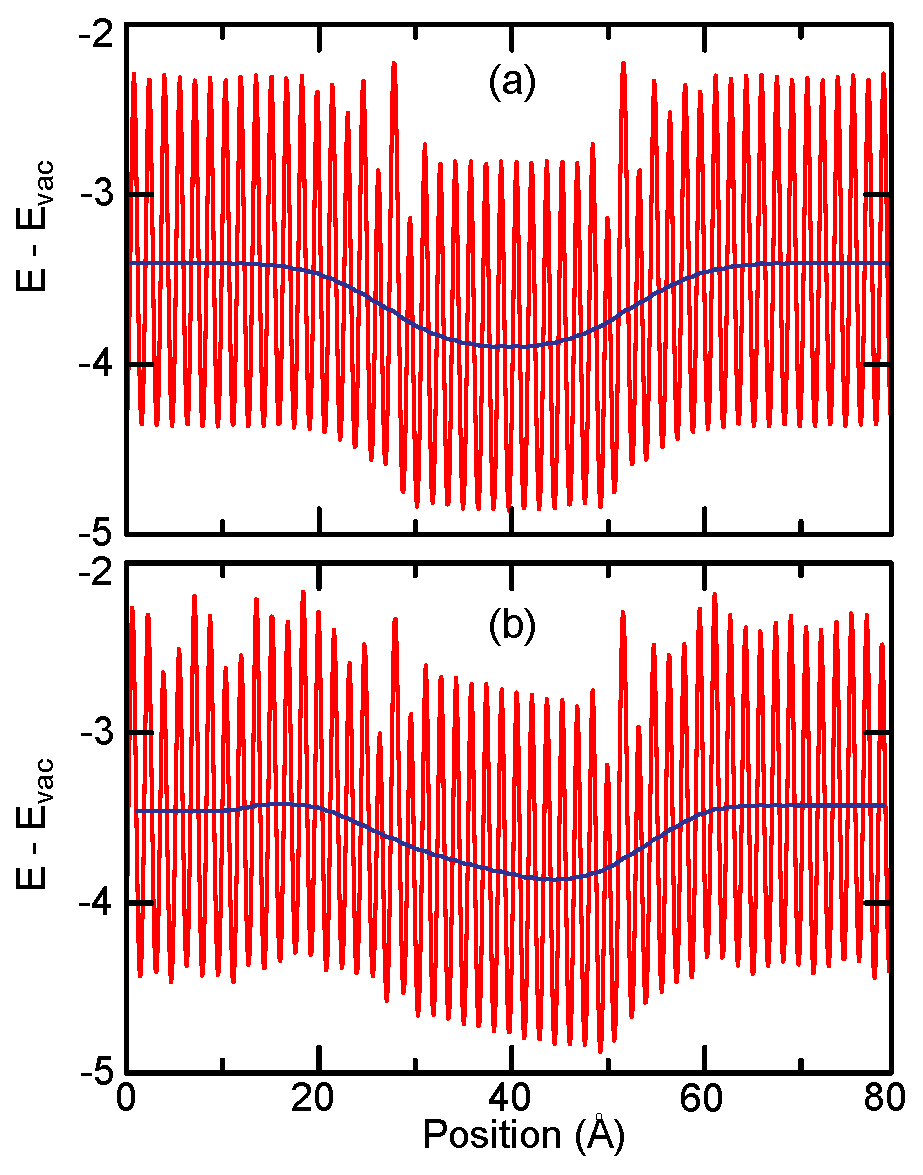
\includegraphics[width=0.8\linewidth]{potential.eps}
\caption{\label{potential}Self-consistent electrostatic potential profile along the interface of armchair (a) pristine and (b) doped 1T$_d$-1H-1T$_d$ MoS$_2$ heterostructure.  The right (left) 1T$_d$ MoS$_2$ is doped with Re (Ta). Blue curve denotes the plane average potential along the heterostructure. }
\end{figure}

\subsubsection{Conclusion}
In this work, we explored the impact of doping on the electronic and charge transport properties across the 1T$_d$-1H MoS$_2$ interfaces by considering various device models. 
Doping and alloying (with charge, atom or molecule) 
appear as an effective method to tailor and improve the physical-chemical properties and stabilities of not 
only 1T/1T$_d$ phases of MoS$_2$ but also other 2D materials. 
The interface structure between 1T$_d$ and 1H phases is one of the decisive factors in the determination of the electrical transport across the heterojunction. 
We found that the Schottky barrier height of electrons for  pristine heterojunctions  can even disappear as a result of electron doping. 
While charge doping only reduces the Schottky barrier for electrons, co-doping is able to tune the barriers for
hole and electrons at the same time.


\section{Defect induction}
\subsection[Faceted blue phosphorene nanotube formed by line defects]{Faceted blue phosphorene nanotube formed by line defects \footcite[This work is published in:][]{Aierken2015.nanotubes}}
